\documentclass[sort&compress, preprint]{elsarticle}
\usepackage[english]{babel}
\usepackage{amsmath,amssymb}
\usepackage{amsthm}
\usepackage{thmtools, thm-restate}
\usepackage{breqn}
\usepackage{bbold}
\usepackage{booktabs}
\usepackage{graphicx}
\usepackage[utf8]{inputenc}
\usepackage[T1]{fontenc}
\usepackage{caption}
\usepackage{siunitx}
\usepackage{hyperref}
\usepackage[labelfont=bf,textfont={sl,bf},lofdepth,lotdepth]{subfig}
\usepackage{xspace}
\usepackage{color}
\usepackage{proba}
\usepackage[usenames,dvipsnames,svgnames,table]{xcolor}
\usepackage{cleveref}
\usepackage{paralist}
\usepackage{todonotes}
\usepackage{bigints}
\usepackage[title,titletoc,toc]{appendix}
\usepackage{import}
\usepackage{natbib}
%%%%%%%%%%%%%%%%%%%%%%%%%%%%%%%%%%%%%%%%%%%%%%%%%%%%%%%%%%%%%%%%%%%%%%%%%%%%%%%%%%%%%%%%%%
%                                  MODIFICACIONES                                        %
%%%%%%%%%%%%%%%%%%%%%%%%%%%%%%%%%%%%%%%%%%%%%%%%%%%%%%%%%%%%%%%%%%%%%%%%%%%%%%%%%%%%%%%%%%
\oddsidemargin=1.0cm
%\evensidemargin=2.0cm
\textwidth=14.5cm
%%%%%%%%%%%%%%%%%%%%%%%%%%%%%%%%%%%%%%%%%%%%%%%%%%%%%%%%%%%%%%%%%%%%%%%%%%%%%%%%%%%%%%%%%%
%                                 FORMATOS                                               %
%%%%%%%%%%%%%%%%%%%%%%%%%%%%%%%%%%%%%%%%%%%%%%%%%%%%%%%%%%%%%%%%%%%%%%%%%%%%%%%%%%%%%%%%%%
%\DeclareMathAlphabet{\mathpzc}{OT1}{pzc}{m}{it}
\theoremstyle{definition}
\newtheorem{definition}{Definition}[section]
\newtheorem{dfn}{Definition}[section]
\newtheorem{assumption}{Assumption}[section]
\newtheorem{hypothesis}{Hypothesis}[section]
%
\theoremstyle{plain}% default
\newtheorem{thm}{Theorem}[section]
\newtheorem{pro}{Proposition}[section]
\newtheorem{lem}{Lemma}[section]
\newtheorem{corollary}{Corollary}[section]
\newtheorem{consequence}{CONSEQUENCE}[section]
\newtheorem{example}{\bf Example}[section]
\theoremstyle{remark}
\newtheorem{remark}{Remark}[section]
\newproof{pf}{Proof}

%declaration theorems for appendix
\declaretheorem[numbered=no, name=H\"{o}lder]{Holder}
\declaretheorem[numbered=no, name=Young]{Young}
\declaretheorem[numbered=no, name=Minkowski]{Minkowski}
\declaretheorem[numbered=no, name=Doob's Martingale Inequality]{Doobs}
\declaretheorem[numbered=no, name=Burkholder–Davis–Gundy inequality]{bdg}
\declaretheorem[numbered=no, name=Gronwall inequality]{Gronwall}
\declaretheorem[numbered=no, name=Discrete Gronwall Inequality]{DiscreteGronwall}
\declaretheorem[numbered=no, name=A standard inequality]{Standard}
%
\providecommand*{\lemautorefname}{Lemma}
\providecommand*{\thmautorefname}{Theorem}
\providecommand*{\assumptionautorefname}{Assumption}
\providecommand*{\hypothesisautorefname}{Hypothesis}
\newcommand{\normL}[1]{\left[\mathbb{E}\left|#1\right|^2\right]^{1/2}}
\newcommand{\ms}[1]{\mathbb{E}\left|#1\right|^2}
\newcommand{\mep}[1]{\mathbb{E}|#1|^p}
\newcommand{\m}[1]{\mathbb{E}#1}
\newcommand{\Prob}[1]{\mathbb{P}\left[#1\right]}
\newcommand{\meanp}[2]{\mathbb{E}\left|#1\right|^{#2}}
\newcommand{\condexp}[2]{\mathbb{E}\left[#1|#2\right]}
\newcommand{\lftrght}[3]{\left#2 #1\right #3}\DeclareMathOperator{\tr}{tr}
\newcommand{\innerprod}[2]{\left\langle#1, #2\right\rangle}
\newcommand*{\eg}{e.g.,\xspace}
\newcommand*{\ie}{i.e.,\xspace}
%\newcommand*{\todo}[1]{\textcolor{BrickRed}{#1}\\}
\newcommand{\crefrangeconjunction}{--}
\crefrangeformat{equation}{(#3#1#4)--(#5#2#6)}
\DeclareMathOperator{\diag}{diag}
\DeclareMathOperator*{\as}{a.s.}
%\DeclareMathOperator{\diag}{diag}
\newcommand{\SM}{LS\xspace}
\AtBeginDocument{\renewcommand{\harvardand}{and}}
\declaretheorem[numberwithin=section]{theorem}
\crefname{hypothesis}{hypothesis}{hypotheses}
\Crefname{hypothesis}{Hypothesis}{Hypotheses}
%
%+++++++++++++++++++++++++++++++++++++++++++++++++++++++++++++++++++++++++++++++++++++++++++++++++++++++++++++
\begin{document}
	\begin{frontmatter}
		\title{
				The Linear Steklov Method
				for SDEs with 
				non-globally Lipschitz Coefficients: Strong convergence and simulation.\tnoteref{t1}
		}%,t2}}
% 		\tnotetext[t1]{
% 			This work has been partially
% 			supported by CONACYT project *****
% 		}
		\author[sj]{S. D\'{\i}az-Infante}
		\ead{sauld@cimat.mx}
		\author[sj]{S. Jerez}
		\ead{jerez@cimat.mx}
		\address[sj]{Split Step Linear Steklov Method 
		Department of Applied Mathematics, CIMAT, Guanajuato, Gto., Mexico,
		36240.
		}
	\begin{abstract}
		We present an explicit  numerical method for
		solving stochastic differential equations  with non-globally Lipschitz
		coefficients. A linear version of the Steklov average under a split-step formulation supports our new solver.
		The Linear Steklov method converges strongly with a standard 
		one-half order.  Also, we present numerical evidence that the explicit 
		Linear Steklov reproduces almost surely stability solutions with  
		high-accuracy for diverse application models  even  for stochastic differential systems 
		with super-linear diffusion coefficients.
	\end{abstract}
	\begin{keyword}
		stochastic differential equations;
		explicit methods; strong convergence; Steklov average.
	\end{keyword}
	\end{frontmatter}
	%\pagebreak
	%\tableofcontents
	%\pagebreak
	
%********************************************************************************************
%              Section 1
%********************************************************************************************

\section{Introduction} 

	Fundamental computational tools in applications,  as Brownian Dynamics \cite{Cruz2012} or Monte Carlo simulations 
\cite{Glasserman2004} requires simple and computational cheap numerical methods  --- 
in some cases this exclude the use of implicit schemes.
In this context, the Euler Maruyama (EM) leads because has simple algebraic structure, 
cheap computational cost and acceptable convergence rate under global Lipschitz condition, but, if the drift or 
diffusion of a SDE grows faster than something linear, then the EM approximation diverges  in mean square sense 
\cite{Hutzenthaler2009, Hutzenthaler2010, Hutzenthaler2012b}.
Moreover, Giles in \cite{Giles2008} proposes an efficient variance reduction technique based on numerical strong 
convergence: the \emph{multilevel}  Monte Carlo method. 
Since applications in Finance, Biology or Physics consider stochastic differential equations (SDE) with super-linear
grow and Locally Lipschitz coefficients as models, designing explicit strong convergent schemes (in $L^p$ sense)
attracts the actual stochastic numerics research. 

	Given its simple structure and low computational, results natural develop numerical schemes (on the
above set up) by improving the EM. In this line arises the tamed schemes
\cite{Hutzenthaler2012a, Hutzenthaler2015, Wang2011, Sabanis2013, Zong2014}, a special type of balanced method 
\cite{Tretyakov2013}, and the stopped scheme \cite{Liu2013a}, which considers local Lipschitz drift and at most linear 
grow diffusion. Recently in \cite{Mao2015} Mao, develops the truncated Euler method and  Sabanis in \cite{Sabanis2015} 
proposes a new tamed type scheme, both considers diffusion, and drift under locally Lipschitz and super-linear grow 
conditions. All of this works  prove  convergence  of their schemes following the theory developed by Higham Stuart and 
Mao in \cite{Higham2002b} or the new approach developed by  Hutzenthaler and Jentzen in \cite{Hutzenthaler2015}.
Both theories turn the problem of prove strong convergence into provide a bound for the moments of the numerical and 
continuous solution of a underlying SDE. The approach of Hutzenthaler and Jentzen provide tools based on conveniently 
rare events while Higham et al. use stopping time techniques.

We consider the  vector It\^o stochastic differential equation (SDE) of the the form
\begin{equation}\label{eqn:SDE1}
	dy(t)
	 =f(y(t))dt + g(y(t))dW(t), \quad 0\leq t\leq T,
	\quad y(0)=y_0,
\end{equation}
where $(f^{(1)},\dots, f^{(d)}):\R^d \to \R^d$ is one sided Lipschitz and 
$g = (g^{(i,j)})_{i\in \{1,\dots,d\}, j\in\{1,\dots, m\}}:\R^d \to \R^{d\times m}$ is global Lipschitz. Also we assume 
that  each component function $f^{(j)}$  has the structure
$$
	f^{(j)}(x) = a_j(x) x^{(j)} + b_j (x^{(-j)}), \qquad x\in \R^d, \qquad 
	x^{(-j)} = \left( x^{(1)},\dots,x^{(j-1)},x^{(j+1)},\dots x^{(d)}\right).
$$ 
Note that Stochastic models as Lotka Volterra, Duffin - Van der Pol, Lorenz, SIR, SIS follow this structure. 
We will work with the standard setup, that is,  $y(t)\in \R^d$ for each $t$ and  $W(t)$ is a
$m$-dimensional standard Brownian motion on a filtered and complete probability space
$
	(
		\Omega ,\calF,(\calF_t)_{t\in[0,T]},\prob{}
	)
$,
with the filtration
$(\mathcal{F}_t)_{t\in[0,T]}$  generated by the Brownian process.
 In this work in order to extend the explicit Steklov method  proposed in \cite{Diaz-Infante2015}  to a multidimensional case   basados en un promedio linealizado  de Steklov \cite{Diaz-Infante2015} .... We  prove order and strong convergence 
  following the work of \citeauthor*{Higham2002b},

In section 2... Section 3 ...

Notation

\section{General Settings}
In this section we remind some classical results  about the moment boundedness, existence 
and uniqueness of the solution of the stochastic differential system \eqref{eqn:SDE1}, 
see \cite{Higham2002b,Mao2013,Mao2007}. Moreover, we state some theorems about the strong 
convergence of the Euler-Maruyama given by Higham et al. in \cite{Higham2002b} which will be useful 
 to prove the strong convergence of the Linear Steklov method. 
 %Finally, 
% we give several definitions and theorems of the multivariable calculus 
% that we consider to justify the existence of the Linear Steklov approximation, 
%  for references \cite{Lawlor2012,FineAIandKass1966}. 
Let us assume
the following:


	
\begin{hypothesis}\label[hypothesis]{ass:OSLC}
	The coefficients of SDE \eqref{eqn:SDE1} satisfy the conditions:
	\begin{enumerate}[({H}-1)]
		\item \label{ass:C1Functions}
		The functions $f,g$ are in the class $C^{1}(\R^d)$.
		\item
		\textbf{Local, global Lipschitz condition}. For each integer $n$, there is a positive
		constant $L_{f}=L_{f}(n)$ such that
		$$
		|f(x)-f(y)|^2 %\vee |g(x)-g(y)|^2
		\leq L_{f}|x-y|^2 \qquad \forall x,y \in \R^d, \qquad |x|\vee|y|\leq n,
		$$
		and there is a positive constant $L_g$ such that
		$$
		|g(x)-g(y)|^2 \leq L_{g}|x-y|^2,
		\qquad  \forall x,y \in \R^d.
		$$ 
		\item\label{ass:MonotoneCondition}
		\textbf{Monotone condition.} There exist two positive constants $\alpha$ and $\beta$
		such that
		\begin{equation}\label{eqn:MonotoneCondition}
		\innerprod{x}{f(x)} +\frac{1}{2}|g(x)|^2
		\leq \alpha +\beta |x|^2, \qquad \forall x \in \R^d.
		\end{equation}
	\end{enumerate}
\end{hypothesis}


Under Hypothesis \ref{ass:OSLC} we can assure  existence and uniqueness 
of the solution of continuous system \eqref{eqn:SDE1}  as well as bounds on its moments
 in order to justify the development of a numerical approximation. Next we enumerate the classical 
 results that we mentioned above.
%
\begin{thm}
	Assume \Cref{ass:OSLC}  then for all $y(0)=y_0\in \mathbb{R}^d$   there exists a 
	unique global solution $\{y(t)\}_{t\geq 0}$ to SDE \eqref{eqn:SDE1}. Moreover, the solution has the 
	following properties for any $T>0$,
	\begin{equation*}
		\ms{y(T)}< 
		\left(
			|y_0|^2 +2\alpha T 
		\right)e^{2\beta T},
	\end{equation*}
	and
	\begin{equation*}
	\Prob{\tau_n\leq T}
	\leq \frac{
		\left(
		|y_0|^2 +2\alpha T 
		\right)
		e^{2\beta T}
	}{n},
	\end{equation*}
	where $n$ is any positive integer and 
	%\begin{equation*}
	$\tau_n := \inf \{ t\geq 0 : |y(t)|>n\}$.
	%\end{equation*}
\end{thm}
%
\begin{thm}
	\label{thm:MaoCoercive}
	Let $p\geq 2$ and $x_0\in L^p(\Omega, \mathbb{R}^d)$. Assume that there exits a constant $C>0$
	such that for all $(x,t)\in \mathbb{R}^d\times [t_0,T]$,
	\begin{equation*}
	\innerprod{x}{f(x,t)}+\frac{p-1}{2}|g(x,t)|^2 \leq C(1+|x|^2).
	\end{equation*}
	Then
	\begin{equation*}
	\m|y(t)|^p
	\leq
	2^{\frac{p-2}{2}}
	\left(
	1 + \m|y_0|^p
	\right)e^{Cpt} \quad \text{ for all } t\in[0,T].
	\end{equation*}
\end{thm}
%
\begin{lem}
	\label{lem:MomentBound}
	Assuming \Cref{ass:OSLC}, for each $p\geq 2$, there is a $C=C(p,T)$ such that
	\begin{equation*}
	\EX{\sup_{0\leq t \leq T}|y(t)|^p}\leq C \left(1+\mep{y_0}\right).
	\end{equation*}
\end{lem}

% Now we  state some  results of the multivariable calculus  like  
% the L'H\^{o}pital Rule and the existence  of the directional derivative 
% at an isolated singularity that will be used  throughout the paper.
% 
% \begin{dfn}
% 	Let $u,\mathbf{q}\in \R^2$ and $\alpha$ the positive angle formed by the $x$-axis and the segment
% 	$\overline{u \mathbf{q}}$.	We denote by 
% 	\begin{align*}
% 		f_{\alpha}(u) &= 
% 			\cos(\alpha) 		
% 			\frac{\partial f}{\partial u^{(1)}}(u) + 
% 			\sin(\alpha)
% 			\frac{\partial f}{\partial u^{(2)}}(u) 
% 			= \frac{ \innerprod{q-u}{\nabla f(u)}}{|u-q|},			
% 	\end{align*}
% 	the $\mathbf{q}$ \emph{directional derivative at $u$}.
% \end{dfn}
% \begin{dfn}
% 	A set $S\subset \R^2$ is \emph{star-like} with respect to a point $\mathbf{q}$, if for each point $s \in S$ the open 
% 	segment $\overline{s \mathbf{q}}$ is in $S$.
% \end{dfn}
% 
% \begin{thm}\label{thm:Lawlor}
% 	Let $\mathcal{N}$ be a neighborhood in $\R^2$ of a point $\mathbf{q}$ for  which
% 	the two differentiable functions $f:\mathcal{N}\to \R$ and $g:\mathcal{N}\to \R$. Set 
% 	$$
% 		C=\{x \in \mathcal{N}: f(x)=g(x)=0 \},
% 	$$
% 	assuming that $C$ is a smooth curve through $\mathbf{q}$ and 	
% 	there exist a vector $\mathbf{v}$ not tangent to $C$ at $\mathbf{q}$
% 	such that the directional derivative $D_{\mathbf{v}}g$ of $g$ in the direction of $\mathbf{v}$ 
% 	is never zero within $\mathcal{N}$ and $\mathbf{q}$ is a limit point of $\mathcal{N}\setminus C$. Then
% 	\begin{equation*}
% 		\lim_{(x,y)\to \mathbf{q}}
% 		\frac{f(x,y)}{g(x,y)} =
% 		\lim_{
% 				\substack{
% 					(x,y)\to \mathbf{q}\\ 
% 					(x,y)\in \mathcal{N} \setminus C
% 				}
% 		}
% 		\frac{D_{\mathbf{v}} f }{D_{\mathbf{v}} g},
% 	\end{equation*}
% 	if the latter limit exists.
% \end{thm}
% 
% 
% 
% \begin{thm}\label{thm:Fine}
% 	Let $\mathbf{q}\in \R^2$ and let $f$,$g$ be functions whose domains include a set $S\subset \R^2$ which is 
% 	star-like 
% 	with  respect to the point $\mathbf{q}$. Suppose that on $S$ the functions are differentiable and that
% 	the directional derivative of $g$ with respect to $\mathbf{q}$ is never zero. With the understanding that all 
% 	limits are taken from within on $S$ at $\mathbf{q}$ and if
% 	$$f(\mathbf{q})=g(\mathbf{q})=0 \qquad \mbox{and} \qquad
% 				\displaystyle
% 				\lim_{x \to \mathbf{q}}
% 				\frac{f_{\alpha}(x)}{g_{\alpha}(x)} = L,$$
% 	then
% 	$$
% 		\lim_{x \to \mathbf{q}}
% 		\frac{f(x)}{g(x)} = L.
% 	$$
% \end{thm}
 Finally, the next theorems gives the necessary conditions to assure strong convergence and 
 the convergence rate of the Euler-Maruyama (EM) 
 method.  
\begin{thm}\label{thm:HighamMaoStuart}
	Assume \Cref{ass:OSLC} holds, then the EM scheme given by: 
	\begin{equation}\label{eqn:EulerMaruyamaHigham}
	Y^{EM}_{k+1}= Y^{EM}_k+hf(Y^{EM}_k) + g(Y^{EM}_k)\Delta W_k,
    \end{equation} 
	where $h$ is the step-size and its
	continuous-time  extension
	\begin{equation}\label{extE}
	\overline{Y}^{EM}(t):=Y_0+\int_0^t f (Y^{EM}_{\eta(s)})\,ds+\int_0^t g(Y^{EM}_{\eta(s)})\,dW(s),
	\end{equation}
	where $\eta(t):=k$ for $t\in[t_k,t_{k+1})$, satisfies
	\begin{equation}
		\lim_{h\to 0}
		\EX{\sup_{0\leq t\leq T}|\overline{Y}^{EM}(t)-y(t)|^2}=0.
	\end{equation}
\end{thm}	
Under the following assumptions, we can get the rate of convergence of the EM scheme.
\begin{hypothesis}\label{PolynomialGrowth}
	There exist positive constants $L_f, D\in \R$ and $q \in \Z^+$ such that $\forall u,v \in \R^d$
	\begin{eqnarray}
		\innerprod{u-v}{f(u)-f(v)}
			&\leq& L_f|u-v|^2, \nonumber \\
		|f(u) - f(v)|^2 
			&\leq& 
				D_f(1 + |u|^q +|v|^q) |u-v|^2,\nonumber
				\\
		|g(u) - g(v)|^2 
			&\leq& 
				D_g(1 + |u|^q +|v|^q) |u-v|^2.\nonumber
	\end{eqnarray}
\end{hypothesis}

\begin{hypothesis}\label{ass:MomentBounds}
	The SDE \eqref{eqn:SDE1} and the EM solution \eqref{eqn:EulerMaruyamaHigham} satisfies
	\begin{equation*}
		\EX{
			\sup_{0\leq t\leq T}
			|y(t)|^p	
		}, \quad
	\EX{
		\sup_{0\leq t\leq T}
			|Y^{EM}(t)|^p	
	}< \infty, \quad
	\EX{
		\sup_{0\leq t\leq T}
		|\overline{Y}^{EM}(t)|^p	
	} < \infty, \qquad \forall p\geq 1.
	\end{equation*}
\end{hypothesis}
\begin{thm}\label{TE}
	Under Hypotheses  \ref{PolynomialGrowth} and \ref{ass:MomentBounds} the EM solution with 
	continuous extension \eqref{extE}
	satisfies
	\begin{equation}
		\EX{
			\sup_{0\leq t \leq T}
			|\overline{Y}^{EM}(t) - y(t)|^2
		} = \mathcal{O}(h).
	\end{equation}
\end{thm}

%********************************************************************************************
%              Section 3
%********************************************************************************************

\section{Construction of the Linear Steklov method} 

\newcommand{\BigFig}[1]{\parbox{12pt}{\Huge #1}}
\newcommand{\BigZero}{\BigFig{0}}
%
In order to construct the LS method, we assume that  for each component of the drift coefficient of \eqref{eqn:SDE1} there exist 
two locally Lipschitz functions $a_j:\mathbb{R}^{d} \to \mathbb{R}$, and
		$b_{j}:\mathbb{R}^{d-1} \to \mathbb{R}$ such that 
		\begin{equation}\label{eqn:AlternativeConstruction}
		f^{(j)}(y) = a_j (y) y^{(j)} + b_{j}(y^{(-j)}), \qquad
		y^{(-j)} = (y^{(1)}, \dots ,y^{(j-1)}, y^{(j+1)}, \dots, y^{(d)}).
		\end{equation}
The Linear Steklov approximation consists in estimating the function $f$ of 
	the SDEs \eqref{eqn:SDE1} (for simplicity $d=j=1$) by 
\begin{equation} \label{ap}
	f(y(t)) \approx 
		\varphi_{f}(y(t_{\eta_{+}(t)})) =
		\left(
			\frac{1}{y(t_{\eta_+(t)})-y(t_{\eta (t)})}
			\int \limits
_				{y(t_{\eta(t)})}^{y(t_{\eta_+(t)})}
					\frac{du}
						{
							a(y(t_{\eta(t)}))u
							+b
						}
	\right)^{-1},
\end{equation}
where  $\eta_+(t):=k+1$ for $t\in[t_k,t_{k+1})$ and $\varphi_f$ 
is the linearized Steklov average \cite{Diaz-Infante2015}. 
Now, using \eqref{ap} we develop the new  method as follows: 
First, let us take  $0=t_0 < t_1< \cdots < t_N=T$ a partition of the interval $[0,T]$ with 
constant step-size $h=T/N$ and such that $t_k=kh$ for $k=0,\ldots, N$.  By discretization
of the SDEs \eqref{eqn:SDE1}, we have for  each component equation $j\in\{1, \ldots,  d\}$ 
	on  the time iteration  $k\in\{1, \ldots,  N\}$, 
	$a_{j,k} =a_j
	\left(
		Y^{(1)}_{k},
		\ldots, Y^{(d)}_{k}
	\right)$  and $b_{j,k} =
	b_{j}
	\left(
			Y^{(-j)}_k
	\right)$. We define the \SM method for 
	the multivariate case under 
a split-step  formulation as:
\begin{eqnarray}
 	Y_{k}^{{\star}^{(j)}} &=& Y_k^{(j)} + h\, \varphi_{f^{(j)}}(Y^{\star}_k), \label{eqn:SSLSM1}\\
	Y_{k+1}^{(j)}	&=& Y_k^{{\star}^{(j)}} + g^{(j)}(Y_k^{\star})\, \Delta W_k 
	\label{eqn:SSLSM2},
\end{eqnarray}
with $Y_0=y_0$ and  $	\varphi_{f}(Y_k^{\star})=
		\left(
			\varphi_{f^{(1)}}(Y_k^{\star}),
			\ldots,
			\varphi_{f^{(d)}}(Y_k^{\star})
		\right)$
where
\begin{equation}\label{fi}
	\varphi_{f^{(j)}}\left(Y_k^{\star}\right)
		=
		\left(
			\frac{1}{Y_{k}^{\star(j)}-Y_{k}^{(j)}}
			\int 
			%\limits
				_{Y_{k}^{(j)}}^{Y_{k}^{\star(j)}}
				\frac{du}
				{
					a_{j,k} u
					+b_{j,k}
				}
		\right)^{-1}.
\end{equation}	
The Linear Steklov algorithmic is an implicit scheme, but 
we can derive an explicit matrix version given by  
\begin{equation}\label{m1}
 Y_{k+1} = A^{(1)}(h,Y_k) \,Y_k + A^{(2)}(h,Y_k)b(Y_k)+ g(Y_k)\, \Delta W_k, 
\end{equation}
where  $A^{(1)}= A^{(1)}(h,u)$,  $A^{(2)}=A^{(2)}(h,u)$   are defined  by
\begin{align}\label{eqn:SolutionFunctions}	
	A^{(1)}&:=
		\begin{pmatrix}
			e^{ha_1(u)} & \multicolumn{2}{c}{\text{\kern0.5em\smash{\raisebox{-1ex}{\Huge 0}}}} \\
			&\ddots\\
			\multicolumn{2}{c}{\text{\kern-0.5em\smash{\raisebox{0.95ex}{\Huge 0}}}} 
			& e^{ha_d(u)}
		\end{pmatrix},
		\notag
		\\
		%	
	A^{(2)}&:=
	\begin{pmatrix}
		\left(
			\displaystyle
			\frac{e^{ha_1(u)} - 1}{a_1(u)}
		\right)\1{E_1^c}% + h \1{E_i}  & 
		&\BigZero\\
		\qquad \qquad \qquad \qquad\ddots&\\
		\BigZero&
		\left(
			\displaystyle
			\frac{e^{ha_d(u)} - 1}{a_d(u)}
		\right)\1{E_d^c}% + h \1{E_i} 
	\end{pmatrix}
	+h
	\begin{pmatrix}
		\1{E_1} & \BigZero\\
		\qquad \qquad \ddots\\
		\BigZero & 
		\1{E_d}
	\end{pmatrix}.	
\end{align}
 and $b(u)=\left(b_1(u^{(-1)}), \dots , b_d(u^{(-d)})\right)^T$.  
It is worth mentioning that the explicit formulation \eqref{m1}-\eqref{eqn:SolutionFunctions} 
is well defined in the set $E_j:=\{x \in \R^d: a_j(x)=0\}$. In the following, we 
assume two important hypotheses which are crucial to prove existence 
of the explicit Linear Steklov method.

\begin{hypothesis}\label[hypothesis]{ass:ajBound} %\label{as:aiFunctions}
	For each component function $f^{(j)}:\R^d:\to \R$, %$j \in \{1, \dots, d \}$,
		$j \in \{1,\dots, d\}$:
	\begin{enumerate}[({A}-1)]
		\item\label{ass:FunctionStructure}
		There are two locally Lipschitz functions of class $C^1(\R^d)$ denoted by
		$a_j:\mathbb{R}^{d} \to \mathbb{R}$ and
		$b_{j}:\mathbb{R}^{d-1} \to \mathbb{R}$ such that 
		\begin{equation*}\label{eqn:AlternativeConstruction}
		f^{(j)}(y) = a_j (y) y^{(j)} + b_{j}(y^{(-j)}), \qquad
		y^{(-j)} = (y^{(1)}, \dots ,y^{(j-1)}, y^{(j+1)}, \dots, y^{(d)}).
		\end{equation*}
		\item\label{a}
		There is a positive constant $L_a$ such that
		\begin{equation*}
		a_{j}(x) \leq L_a, \qquad \forall x\in \R^d, \quad j=1,\ldots, d.
		\end{equation*}
		\item Each function $b_j(\cdot)$ satisfies the linear growth condition
		\begin{equation*}\label{eqn:bjLinearGrowthCondition}
		|b_j(u^{(-j)})|^2 \leq L_{b}(1+|u|^2) , \qquad \forall x\in \R^d, \quad j=1,\ldots, d.
		\end{equation*}
		\item For each $x\in E_j$ there is an open ball of positive 
		radius and center $x$, $B_r(x)$, such that 
		$$
		\frac{\partial a_j(u)}{\partial u^{(j)}}
		\neq 0, \qquad \forall u \in B_r(x) \setminus E_j.
		$$
	\end{enumerate}
\end{hypothesis}
\begin{hypothesis}\label{ass:HypThmSingularities}
	The set $E_j:=\{x\in \R^{d}: a_j(x)=0\}$ satisfies either:
	\begin{enumerate}[(i)]
		\item  All points of  $ x\in E_j$  which are non isolated zeros of $a_j$ and:
			\begin{itemize}
				\item The set $D_x:=\{u \in B_r(x): a_j(u)= 0\}$ 
					is a smooth curve through $x$. 
				\item
					The canonical vector $e_j$ is not
					tangent to $D_x$.
				\item
					For each $x \in E_j$, there is an open ball with center
					on $x$ and radio $r$, $B_r(x)$, such that  
					$$
						a_j\neq 0, \qquad
						\frac{\partial a_j(u)}{\partial u^{(j)}} \neq 0 ,\qquad 
						\forall u \in B_r(x)
						\setminus D_x.
					$$	
			\end{itemize}	
		\item
			All points $x \in E_j$ which are isolated zeros of $a_j$ and:
			\begin{itemize}
				\item
					For each $x\in E_j$,  $x$ is not a limit point of the set 
					$E_{\alpha}:=\{u \in \R^d: (a_j)_\alpha(u)=0\}$.
				\item
					For each $x \in E_j$, there is a subset $E_x$ such that the open segment 
					$\overline{x\,u}$ is in $E_x$ and 
					the $x$ directional derivative at $u$ satisfies
					$$
						 (a_j)_\alpha(u) \neq 0, \qquad \forall u\in E_x.
					$$
			\end{itemize}		
	\end{enumerate}	
\end{hypothesis}
Hypothesis \ref{ass:HypThmSingularities} assures  the existence of the directional derivative at an isolated 
singularity, for references \cite{Lawlor2012,FineAIandKass1966}. Under the previous  assumptions, 
we will show that the explicit Linear  Steklov approximation \eqref{m1}-\eqref{eqn:SolutionFunctions} always 
exists, the function $\varphi$ is bounded by the drift function $f$ and also the 
coefficients $\varphi$  and $g$  satisfy a monotone condition. First, we will give a lemma.
\begin{lem}\label{l1}
 Assume \Cref{ass:OSLC,ass:ajBound,ass:HypThmSingularities} hold. The function $\Phi_j(u)=\Phi(h, a_j)(u)$ 
 defined by
 \begin{equation}\label{eqn:ExpBound}
		\Phi_j(u):=\frac{e^{ha_j(u)}-1}{ha_j(u)},
	\end{equation}
	is bounded  on $\R^d$ for each $j\in \{ 1,\dots, d\}$ 
	and we denote its bound by $L_{\Phi}$.
\end{lem}
\begin{pf}    By \Cref{ass:OSLC}, the operator $\Phi$ is continuous
	on $E_j^c$, thus 
	\begin{equation}\label{e0}
		\lim_{h\to 0}
		\frac{e^{ha_j(u)}-1}{ha_j}=1,
	\end{equation}
	for each fixed $u\in E_j^c$. If $u^*\in E_j$ and fixing any $h$, by \Cref{ass:HypThmSingularities}, 
	we obtain one of the following cases:
	\begin{equation}\label{eqn:ajSingularityCasei}
				\lim_{
					\substack{
						u \to u^*\\ 
						u\in E_j^c
					}
				}
				\Phi(h,a_j)(u) =
				%
				\lim_{
					\substack{
						u \to u^*\\ 
						u\in E_j^c
					}
				}	
				\frac{\frac{\partial a_j(u)}{\partial u^{(j)}} 
					h e^{h a_j(u)} 
				}{
					h\frac{\partial a_j(u)}{\partial u^{(j)}}
				}=1,
			\end{equation}	
or
			\begin{equation}\label{eqn:ajSingularityCaseii}
			\lim_{
				\substack{
					u \to u^*\\ 
					u\in E_j^c
				}
			}
			\Phi(h,a_j)(u) 
			=
			%
			\lim_{
				\substack{
					u \to u^*\\ 
					u\in E_j^c
				}
			}	
			\frac{
				\left(
					 e^{h a_j(u)} - 1
				 \right)_{\alpha}
			}{
				\left(
					h a_j(u)
				\right)_{\alpha}
			}	=	1, \qquad \alpha = 0,\pi, 2\pi,\dots
		\end{equation}	
	From \eqref{e0}, \eqref{eqn:ajSingularityCasei} and \eqref{eqn:ajSingularityCaseii} we can deduce that 	
	\begin{equation}\label{eqn:PhiBound}
		\left|\frac{e^{ha_j(u)}-1}{ha_j(u)}
		\right|\leq\left|\frac{e^{hL_a}-1}{ha^*_j}
		\right|,
		\qquad \forall u \in \R^d.
	\end{equation}
	where $a^*_j:= \inf_{u\in E_j^c}\{|a_j(u)|\}$. Even though $a^*_j=0$, we can
	use an argument similar to \crefrange{eqn:ajSingularityCasei}{eqn:ajSingularityCaseii}.	\qed	
\end{pf}

We can  now state the following theorem.

\begin{thm}\label{lem:PhiFhProp}
	Assume \Cref{ass:OSLC,ass:ajBound,ass:HypThmSingularities} hold, and $A^{(1)}$, $A^{(2)}$, $b$  
	defined by 
	\eqref{eqn:SolutionFunctions}. Then given $u\in\mathbb{R}^d$, the equation
	\begin{equation}\label{eqn:varphiEquation}
		v = u + h \varphi_f(v),
	\end{equation}
	has a unique solution 
	\begin{equation}\label{eqn:varphiEqnSolution}
		v = A^{(1)}(h,u)u +A^{(2)}(h,u) b(u)	.
	\end{equation}
%
	If we define the functions
	$F_h(\cdot)$, $\varphi_{f_h}(\cdot)$ and $g_h(\cdot)$ by
	\begin{equation}\label{eqn:FunctionshDefinition}
		F_h(u) = v,
%			\left(
%				u + \frac{b}{a(u)}
%			\right)\exp\left(ha(u)\right)
%				-\frac{b}{a(u)},
			\qquad 
			\varphi_{f_h}(u) =\varphi_{f}(F_h(u)),
			\qquad
			g_h(u) = g(F_h(u)),
	\end{equation}
	then $F_h(\cdot)$, $\varphi_{f_h}(\cdot)$, $g_h(\cdot)$ are local Lipschitz functions 
	and for all $u\in \mathbb{R}^d$ and each $h$ fixed, there is a positive constant $L_{\Phi}$ such that
	\begin{equation}\label{eqn:PhifhFbound}
		|\varphi_{f_h}(u)|\leq L_{\Phi} |f(u)|. 
	\end{equation} 
	Moreover, for each $h$ fixed,
	%$g_h$ is a locally Lipschitz function and 
	 there are positive constants $\alpha^*$ and  $\beta^*$ such that
	\begin{equation}\label{eqn:h-MonotoneCondition}
		\innerprod{\varphi_{f_h}(u)}{u} \vee |g_h(u)|^2 \leq \alpha^* + \beta^* |u|^2, 
		\qquad
		\forall u \in \R^d.
	\end{equation}
\end{thm}
%
\begin{pf}
	%\todo{Justify the uniform convergence of  $\varphi_{f_h}$ and $g_h$.}
	Let us first prove that \eqref{eqn:varphiEqnSolution} is solution 
	of equation \eqref{eqn:varphiEquation}.  Note that 
	\begin{equation}\label{e1}
		v^{(j)} = u^{(j)} + h \,\varphi_{f^{(j)}}(v),	
	\end{equation}
	for each $j\in \{1,\dots, d\}$ and using the linear Steklov function \eqref{ap}, 
	 we can derive that
	\begin{equation}
		v^{(j)}= e^{h a_j(u)} u^{(j)} + 
		\left[
			h\Phi_j(u)
			\1{E_j^c}
			+h \1{E_j}
		\right]b_{j}(u^{(-j)}),
	\end{equation}	
	 which is the $j$-component of the vector
	$A^{(1)}u +A^{(2)} b(u)$. Now we prove inequality \eqref{eqn:PhifhFbound}. Given that 
	$v =\varphi_{f}(F_h(u))$, 
	we can also rewrite \eqref{e1} as
	$$
		\varphi_{f_h}^{(j)}(u) = 
			\frac{
%				\displaystyle
				F_h^{(j)}(u)-u^{(j)}
			}%
			{%				
				\displaystyle
				\int_{u^{(j)}}^{F_h^{(j)}(u)}
				\frac{dz}{a_j(u)z + b_j(u^{(-j)})}
			}.
	$$
	If $u\in E_j$ then $\varphi_{f_h}^{(j)}(u) = b_j(u^{(-j)}) = f^{j}(u)$,
	so $L_{\Phi}\geq 1$ fulfills  \eqref{eqn:PhifhFbound}.
	On the other hand, if $u\in E_j^c$ then
	\begin{equation}\label{eqn:VarPhiEjc}
		\varphi_{f_h}^{(j)}(u) =
		\frac{
				(F_h^{(j)}(u)-u^{(j)}) a_j(u)
			}
			{
				\underbrace{
				\ln \left(
					a_j(u) F_h^{(j)}(u) + b_j(u^{(-j)})
				\right)
				}_{:=R_1}
				-
				\ln \left(
					a_j(u) u^{(j)} + b_j(u^{(-j)})
				\right)
			}=\Phi_j(u)f^j(u),		
	\end{equation}
	 where
	\begin{equation}\label{eqn:Ter1Simplification}	
		R_1=
			\ln\left\{
				a_j(u)\left[
					e^{ha_j(u)}u^{(j)} +
					h\Phi_j(u) b_j(u^{(-j)})	
				\right]
				+b_j\left(u^{(-j)}\right)
			\right\} \notag \\
		=h a_j(u) + \ln \left( f^{(j)}(u) \right).		
	\end{equation}
	By lemma \ref{l1}, inequality \eqref{eqn:PhifhFbound} is satisfied 
	for all $u\in E_j \cup E_j^c$. 	As $g_h(x)=g\left(F_h(x) \right)$, 
	by \Cref{ass:OSLC}, then
	\begin{equation} \label{eqn:gLocalLipschitzArg} 
		|g_h(u)-g_h(v)|^2 \leq
			L_g|F_h(u)- F_h(v)|^2  \leq
			2L_g \underbrace{
				|A^{(1)}u - A^{(1)}v|^2 
			}_{:=R_2} +
			2L_g \underbrace{
				|A^{(2)}b(u) - A^{(2)}b(v) |^2 
			}_{:=R_3}.			
	\end{equation}
	Let us consider each term of the right hand of inequality \eqref{eqn:gLocalLipschitzArg}.
	First, note that $A^{(1)}$ is a continuous differentiable function on all 
	$\R^d$, so using the mean value theorem,
	we have
	\begin{equation}\label{eqn:BoundTer1gh}
		R_2
		\leq
		L_{A^{(1)}}|u-v|^2, \quad u,v \in \R^d, \quad |u|\vee |v|\leq n,
	\end{equation}
	for a positive constant $L_{A^{(1)}} \geq \sup_{0\leq t \leq 1} 
		|\partial A^{(1)}(h, u+t(v-u))|^2$. Meanwhile, 
	\begin{eqnarray}
	R_3 &=&\sum_{j=1}^d\Big[\1{E_j^c}(u) \Phi_j(u) b_j(u^{(-j)}) + h \1{E_j}(u) b_j(u^{(-j)}) 
			-\1{E_j^c}(v) \Phi_j(v) b_j(u^{(-j)})\nonumber \\ &-& h \1{E_j}(v) b_j(v^{(-j)})
			\Big]^2 
			\leq
			4\sum_{j=1}^d
			\Big[
				\left(	
					\1{E_j^c}(u) L_{\Phi} b_j(u^{(-j)})  
				\right)^2
				+
				\left(
					h \1{E_j}(u) b_j(u^{(-j)})
				\right)^2
				\nonumber\\&+&
				\left(
					\1{E_j^c}(v) L_{\Phi} b_j(v^{(-j)})
				\right)^2
				+
				\left(
				 h \1{E_j}(v) b_j(v^{(-j)}
				\right)^2
			\Big].
		\label{eqn:BoundArgTer2}	
	\end{eqnarray}	
	Since  $b^2_j(\cdot)$ is a function of class $C^1(\R^d)$, there is a 
	constant $L_b=L_b(n)$ such that
	\begin{dmath}[label={eqn:Boundbju}]
		|b_j(u)|^2 \leq L_b 
		\condition{
			$\forall u \in \R^d$,
			\quad $|u| \vee |v| \leq n$,}		
	\end{dmath}
	for each $j \in \{1,\cdots, d\}$. Using this bound in  \eqref{eqn:BoundArgTer2}, we obtain
	\begin{equation}\label{eqn:BoundL0Ter2gh}
			R_3\leq
			4 \sum_{j=1}^d
				\left[
					2 L_{\Phi} L_b +2h^2 L_b
				\right] 
			\leq L_0, \qquad
				\forall u,v \in \R^d,
				\quad |u|\vee|v| \leq n,
	\end{equation}
	where $L_0=8d L_b(n)(L_{\Phi}+h^2)$.
	By inequalities \eqref{eqn:BoundTer1gh} and \eqref{eqn:BoundL0Ter2gh},  we get
	\begin{equation}
			|g_h(u) - g_h(v)|^2 \leq L_{g_h}(n) |u - v|^2, 
			\qquad	\forall u,v \in \R^d,
				\quad |u|\vee |v| \leq n,		
	\end{equation}
	 where $L_{g_h}(n)\geq n^2+1+L_0+ L_{A^{(1)}}$. Then $g_h(\cdot)$ is a locally 
	 Lipschitz function. Furthermore, note that under some modifications
	this argument can be used to prove that $F_h(\cdot)$ is also a locally Lipschitz 
	function, which implies that $\varphi_{f_{h}}$ is a locally Lipschitz function.
	Finally, we  will demonstrate inequality \eqref{eqn:h-MonotoneCondition}. 
	By \Cref{ass:OSLC,ass:ajBound}, we have
	\begin{equation*}\label{eqn:bDotProdBound}
			\innerprod{f(u)}{u}
			=
			\sum_{j=1}^d
				a_j(u) \left( u^{(j)} \right)^2
			+
			\sum_{j=1}^d
			b_j(u) u^{(j)}
			\leq \alpha +\beta |u|^2,
	\end{equation*}
	and
		\begin{equation*}\label{eqn:bDotProdBound}
			\innerprod{b(u)}{u} \leq \alpha + (\beta + L_a)|u|^2.
		\end{equation*}
	Using these inequalities and \eqref{eqn:PhifhFbound}, we deduce that
	\begin{equation}\label{eqn:VarphifhDotProdBound}
			\innerprod{\varphi_{f_h}(u)}{u} 
				=\sum_{j=1}^d
						\Phi_j(u) f^{(j)}(u) u^{(j)}
				\leq L_{\Phi} L_a|u| +  L_{\Phi}(\alpha + (L_a + \beta)|u|^2) \leq
				L_{\varphi_{f_h}} (1+|u|^2).					
		\end{equation}
	where
	$
		L_{\varphi_{f_h}}\geq 2 L_{\Phi}\max\{L_a, \alpha, \beta\} + 1.
	$ 
	Meanwhile, since $g$ is globally Lipschitz then
	\begin{equation}\label{eqn:GloballyLipg}
		|g_h(u)|^2 
		\leq
			2 |g(F_h(u)) - g(F_h(0))|^2  + 2 | g(F_h(0))|^2 \leq
			4 L_g |F_h(u)|^2  + 8 L_g |F_h(0)|^2  + 4 |g(0)|^2 .
	\end{equation}
	Now, we bound each term on the right-hand side of  \eqref{eqn:GloballyLipg}.
	By the monotone condition \eqref{eqn:MonotoneCondition}, $|g(0)|^2 \leq 2\alpha$.
	Moreover,
	\begin{equation*}
		|F_h^{(j)} (0) |=
			h\Phi_j(0)\,| b_j(0)| \1{E_j^c}(0) + 
			h\,|b_j(0)| \1{E_j}(0)
			\leq
			\frac{b_0^*}{a_0^*}
			e^{h L_a} (1+h),
			\quad
			\forall j \in \{1, \cdots, d\}.
	\end{equation*}
	where
	$a^*_0 := 
			\min_{
				\substack{
					j \in \{1, \cdots, d \}\\
					a_j(0) \neq 0
				}
			}
			\left\{
				|a_j(0)|
			\right\}$
 and 
		$b^*_0 :=
			\max_{\substack{
				j\in \{1,\cdots, d\}}
			}
			\left\{
				|b_j(0)|
			\right\}.$
	Then
	\begin{equation} \label{eqn:BoundFhZero}
		|F_h(0)|^2 
			\leq
			d\left(
				\frac{b_0^*}{a_0^*}
			\right)^2
		e^{2h L_a} (1+h)^2.
	\end{equation}
	As $\Phi_j$ is bounded, we get
	\begin{dmath*}
		F_h^{(j)}(u) 
			=
			e^{h a_j(u)} u^{(j)} +
			h \Phi_j(u) b_j(u) \1{E_j^c}(u) +h b_j(u) \1{E_j}(u)
			\leq
			e^{h a_j(u)} |u^{(j)}| +
			h L_{\Phi} |b_j(u)| \1{E_j^c}(u) +h |b_j(u)| \1{E_j}(u).
	\end{dmath*}
	 And by \Cref{ass:ajBound},
	\begin{eqnarray}
		|F_h^{(j)}(u)|^2 
		&\leq&
			3 e^{2h L_a }|u|^2 + (3 h^2 L_{\Phi}^2 L_b + 3h^ 2L_b) (1+|u|^2) \nonumber\\
		&\leq&
			3 h^2 L_b (1 + L_{\Phi}^2)   +
			3 \left(
				 e^{2 h L_a} + h^2 L_b (L_{\Phi}^2 + 1 ) 
			\right)|u|^2 \nonumber\\ &\leq& L_F(1+|u|^2), \label{eqn:BoundFhu}
	\end{eqnarray}
	where
	$L_F\geq 3 d \max\{e^{2h L_a},  h^2 L_b(L_{\Phi}^2+1)\}$.
	Using \eqref{eqn:BoundFhZero} and \eqref{eqn:BoundFhu} in  inequality \eqref{eqn:GloballyLipg} yields
	\begin{equation*}
		|g_h(u)|^2 \leq
			4 L_g L_F(1+|u|^2)
			+ 8 L_g d
			\left(
				\frac{b_0^*}{a_0^*}
			\right)^2
			e^{2h L_a} (1+h)^2
			+8 \alpha.
	\end{equation*}
	Therefore, taking
	$
		 L_{g_h} 
		 \geq 
			  4 L_g L_F + 8 L_g d
			  \left(
				  \frac{b_0^*}{a_0^*}
			  \right)^2
			  e^{2h L_a} (1+h)^2
			  +8 \alpha		  
	$
	then
	\begin{equation}\label{eqn:Boundghu}
		|g_h(u)|^2
		\leq
			L_{g_h}(1+|u|^2).		
	\end{equation}
	Hence, from inequalities \eqref{eqn:VarphifhDotProdBound} and \eqref{eqn:Boundghu} 
	and taking for each fixed $h>0$, $\alpha^* := L_{\varphi_{f_h}}\vee L_{g_h}$ and
	$\beta^* := 2\alpha^*$, we obtain inequality  \eqref{eqn:h-MonotoneCondition}.\qed
\end{pf}
%
\begin{remark}\label{rmk:PertrubedSDE}
	It is worth mentioning that if $b_j=0$ in (A-1) 
	then Hypotheses \ref{ass:ajBound} and \ref{ass:HypThmSingularities} are unnecessary to 
	prove \Cref{lem:PhiFhProp}. Several  applications  as  stochastic
	Lotka-Volterra systems \cite{Mao2002,Mao2003},  
	the Ginzburg-Landau SDE \cite{Kloeden1992} or
	the damped Langevin Equations where the potential lacks of a constant term 
	(for example $U(x) = \frac{1}{4}|x|^4 - \frac{1}{2}|x|^2$) \cite{Hutzenthaler2012a}.
\end{remark}

Theorem \ref{lem:PhiFhProp} holds the key to demonstrate strong convergence of the explicit LS method. 

\section{Strong Convergence of the Linear Steklov Method} 

 To prove strong convergence of the Linear Steklov method \eqref{m1}-\eqref{eqn:SolutionFunctions} for  
SDEs with locally Lipschitz coefficients, we rely on the Higham-Mao-Stuart (HMS) technique  
 \cite{Higham2002b}. Recently, several works have used  this  procedure  
 to establish strong convergence for some particular scheme among others \cite{Beyn2010,Guo2014,Hutzenthaler2015,Hutzenthaler2012a,Hutzenthaler2010,Lamba2007,
 Mao2013,Tretyakov2013}. The proof is rather technical and can be divided into the following steps:
 
 \begin{enumerate}[\bf{Step} 1:]
 	\item The explicit LS method \eqref{m1}-\eqref{eqn:SolutionFunctions} is equivalent to 
 	the Euler-Maruyama method \eqref{eqn:EulerMaruyamaHigham} 
	for the conveniently modified SDE
	\begin{equation} \label{eqn:PerturbedHighamSDE}
		dy_h(t)= \varphi_{f_h}(y_h(t))dt +g_h(y_h(t))dW(t),
		\qquad y_h(0)=y_0,  \qquad t\in [0,T],
	\end{equation}
	which is a perturbation of SDE \eqref{eqn:SDE1} given that $|f(x)-\varphi_{f_h}(x)|=\calO(h)$.
	\item\label{stp:PerturbedSolution}
			The solution of the modified SDE \eqref{eqn:PerturbedHighamSDE} has 
			bounded moments and it is 
			"close" to  the solution of the SDEs \eqref{eqn:SDE1}  in the sense of the uniform mean square norm 
			$
				\EX{\sup_{0\leq t\leq T}|\cdot|^2}
			$.
	\item
	\label{stp:MethodBoundedMoments}
		The explicit LS method  has bounded moments.
	\item
		There is a continuous extension of the explicit LS method of the form: 
		\begin{equation}\label{contLS}
		\overline{Y}(t):=Y_0+\int_0^t\varphi_{f_h}(Y_{\eta(s)})\,ds+\int_0^t g(Y_{\eta(s)})\,dW(s), 
		\end{equation}
		where $\eta(t):=k$ for $t\in[t_k,t_{k+1})$, which has bounded moments.
	\end{enumerate}	
	Proving the above statements and using theorem \ref{thm:HighamMaoStuart},
	we can conclude the strong convergence of the explicit LS method. 
	Step 1 is formalized in the following corollary.
	
%======================================================================================================================
%                                                 STEP 1                                                              %
%======================================================================================================================

\begin{corollary}\label{col:SSSMeEMmod}
	Assume \Cref{ass:OSLC,ass:ajBound,ass:HypThmSingularities} hold, then the 
	explicit \SM method \eqref{m1}-\eqref{eqn:SolutionFunctions} for SDE \eqref{eqn:SDE1} is 
	equivalent to the Euler-Maruyama scheme applied to the modified SDE \eqref{eqn:PerturbedHighamSDE}.
\end{corollary}
\begin{pf}
	Using the functions $\varphi_{f_h}(\cdot)$ and $g_h(\cdot)$ defined in \eqref{eqn:FunctionshDefinition}, 
	we can rewrite the explicit \SM method  as 
	$$
		Y_{k+1} = Y_k + h \varphi_{f_h}(Y_k) + g_h(Y_k)\Delta W_k,
	$$
	which is the EM approximation for the modified SDE \eqref{eqn:PerturbedHighamSDE}. \qed
\end{pf}
%======================================================================================================================
%                                                 STEP 2                                                              %
%======================================================================================================================

	Now we proceed with step 2. 
\begin{lem}\label{lem:BoundAndConvergenceOfyh}
	Assume \Cref{ass:OSLC,ass:ajBound,ass:HypThmSingularities} hold, then there is a universal 
	constant $C=C(p,T)>0$ and a sufficiently small
	step size $h$, such that for all $p>2$
	\begin{equation}\label{eqn:yh-MomentBounds}
		\m\left[
			\sup_{0\leq t \leq T}
				|y_h(t)|^p
		\right]
		\leq
			C
		\left( 
			1+\m |y_0|^p
		\right).
	\end{equation}
	Moreover
	\begin{equation}\label{eqn:yh-convergence}
	\lim_{h \to 0}
	\m\left[
	\sup_{0\leq t \leq T}
	|y(t)-y_h(t)|^2
	\right]=0.
	\end{equation}
\end{lem}
\begin{pf}
	By theorem \ref{thm:MaoCoercive} and inequality \eqref{eqn:h-MonotoneCondition}, 
	we have	 bound \eqref{eqn:yh-MomentBounds}.
	On the other hand, to prove \eqref{eqn:yh-convergence} we will use the properties of 
	$\varphi_{f_h}$ and the Higham's stopping time technique employed in \cite[Thm 2.2]{Higham2002b}. 
	Note that by relationship \eqref{eqn:VarPhiEjc}, we can rewrite the Steklov function  as
	\begin{align}\label{fo}
		\varphi_{f_h}(u) 
			&=  f^{(j)}(u) \1{E_j}(u) +\Phi_j(u) f^{(j)}(u) \1{E_j^c}(u) .
	\end{align}
	 If $u\in E_j^c$, given that  $f \in C^1(\R^d)$ and  
	$\Phi_j(\cdot)$ is a bounded function,
	there is a positive constant $K_n$, which depends on $n$, such that 
	\begin{align*}	
		|\varphi_{f_h}^{(j)}(u) - f^{(j)}(u)|
		&\leq
			\1{E_j^c}(u)
			|f^{(j)}(u)|
			\left|
				\Phi_j(u) - 1
			\right| \notag \\
		&\leq
			\1{E_j^c}(u)
			\left(
				L_{\Phi} + 1
			\right)
			|f(u)|	 \notag \\
		&\leq
		\1{E_j^c}(u) K_n(L_{\Phi}+1), \quad \forall u \in \R^d, \quad |u|\leq n,
	\end{align*}
	for each $j\in \{1,\dots, d\}$. At the interface betweeen $E_j$ and $E_j^c$, 
	we know by the scalar L' H\^{o}pital theorem that 
	$ \lim_{h\to 0} \Phi_j(u) = 1$ for $u\in E_j^c$.
	And if $u\in E_j$,  by \Cref{ass:HypThmSingularities} and using   
	theorems \ref{thm:Lawlor} and \ref{thm:Fine}, we have 
	\begin{equation*}
	\lim_{h \to 0} F_h^{(j)}(u)
		=
		\lim_{h \to 0}
			e^{ha_j(u)} u^{(j)} + 
		\lim_{h \to 0}
			\left( \Phi_j(u)
				\1{E_j^c}(u)
				+h \1{E_j}(u)
			\right)
			b_j(u^{(j)}) 
		= u^{(j)},
	\end{equation*}
	for each $j \in \{1, \dots , d\}$, hence
	$%\begin{equation*}
		\displaystyle
		\lim_{h\to 0} F_h(u)=u.
	$ %\end{equation*}
	Consequently, given $n>0$ there is  a function $K_n(\cdot):(0,\infty)\to (0,\infty)$ such that
	$K_n(h)\to 0$ when $h \to 0$ and
	\begin{equation}\label{eqn:PhihGhKRhBound}
		|\varphi_{f_h}(u)-f(u)|^2 \vee |g_h(u)-g(u)|^2
		\leq K_n(h) \qquad \forall u\in \R^d, \quad |u| \leq n.
	\end{equation}
	Meanwhile, since $f$, $g$ are $C^{1}$ there is  a constant $H_n>0$ such that
	\begin{equation}\label{eqn:f-gHRBound}
		|f(u)-f(v)|^2 \vee |g(u)-g(v)|^2
		\leq H_n |u-v|^2\qquad \forall u,v \in \R^d, \quad|u|\vee |v| \leq n.
	\end{equation}
	Now, using the stopping time technique given in \citep[Lem. 3.6]{Higham2002b},  we
 get the desired conclusion.\qed
\end{pf}

%======================================================================================================================
%                                                 STEP 3                                                              %
%======================================================================================================================
In the following, we proceed with step 3 which establishes that \SM method has bounded moments. 
This is  the key step in the HMS technique.


\begin{lem}\label{lem:SSSMMomentBounds}
	Assume \Cref{ass:OSLC,ass:ajBound,ass:HypThmSingularities} hold, then for each $p\geq 2$ there is 
	a universal positive constant 
	$C=C(p,T)$ 
	such that for the explicit \SM method \eqref{m1}-\eqref{eqn:SolutionFunctions} is satisfied
	\begin{equation*}
		\m\left[
		\sup_{kh \in [0,T]}
		|Y_k|^{2p}
		\right]\leq C.
	\end{equation*}
\end{lem}
\begin{pf}
	Using a split formulation of the \SM scheme \eqref{m1}-\eqref{eqn:SolutionFunctions} as follows:
	\begin{eqnarray*}
 	Y_{k}^{{\star}^{(j)}} &=& A^{(1)}(h,Y_k) Y_k + A^{(2)}(h,Y_k) b(Y_k), \label{split1}\\
	Y_{k+1}^{(j)}&=& Y_k^{{\star}^{(j)}} + g^{(j)}(Y_k^{\star})\, \Delta W_k 
	\label{split2},
\end{eqnarray*}
	from the first step of this split scheme, using (A-3) and 
	the Cauchy-Schwartz inequality, we get
	\begin{eqnarray}
		|Y_k^{\star}|^{2}
		&\leq&
			|A^{(1)}(h,Y_k)|^2 |Y_k|^2  
			+ 2 \innerprod{A^{(1)}(h,Y_k)Y_k}{A^{(2)}(h,Y_k) Y_k b(Y_k)}
			+|A^{(2)}(h,Y_k)|^2 |b(Y_k)|^2\nonumber\\
		&\leq&
			|A^{(1)}(h,Y_k)|^2 |Y_k|^2  
		+ 2 \sqrt{L_b} d|A^{(1)}(h,Y_k)||A^{(2)}(h,Y_k)||Y_k|(1+|Y_k|)
		\label{leqn:Yn2Bound} 
		\\& & +L_b|A^{(2)}(h,Y_k)|^2 (1+|(Y_k)|^2). \nonumber
	\end{eqnarray}
	From (A-2), we can deduce that
	\begin{dmath}[label=eqn:A1Bound]
		|A^{(1)}(h,Y_k)|^2 
		=
			\left|
				\diag
				\left(
					e^{ha_1(Y_k)}, \dots, e^{ha_d(Y_k)} 
				\right)
			\right|^2
		\leq M_{A^{(1)}},		
	\end{dmath}
	where $M_{A^{(1)}}=d\, e^{ 2 T L_a}$ and also by \eqref{eqn:PhiBound}, we can derive that
	\begin{align}
		|A^{(2)}(h,Y_k)|^2 
		&=
		\left|
			h 
			\diag
			\left(
				\1{E_1}(Y_k)
				+\1{E_1^c}(Y_k)\Phi_1(Y_k), 
				\dots,
				\1{E_d}(Y_k)
				+\1{E_d^c}(Y_k) \Phi_d(Y_k)
			\right)
		\right|^2 \notag \\
		%
		&\leq
		\sum_{j=1}^{d}
		\left(
			\1{E_j^c}
			|h\Phi_j(Y_k)|^2
			+ h^2
		\right)
		\leq
		2 e^{2 L_a  T}
				\sum_{j=1}^d
				\frac{1}{a_j^*} + d T^2\leq M_{A^{(2)}}.
		\label{eqn:A2Bound}
	\end{align}
	Substituting \eqref{eqn:A1Bound} and \eqref{eqn:A2Bound}  on  inequality \eqref{leqn:Yn2Bound} yields
	\begin{eqnarray}\label{eqn:YkStarBound}
		|Y_k^{\star}|^2
		&\leq&	L_{A^{(1)}} |Y_k|^2
			+ 2 d \sqrt{L_{A^{(1)}} L_{A^{(2)}} L_b }\,|Y_k|(1+|Y_k|)
			+L_{A^{(2)}} L_b (1+|Y_k|^2) \nonumber\\
			&\leq& 
				\widetilde{C}(3|Y_k|^2+|Y_k| + 1) 			
			\leq C(1+|Y_k|^2),
	\end{eqnarray}
	where $\widetilde{C}\geq L_{A^{(1)}}+ 2 d \sqrt{L_{A^{(1)}} L_{A^{(2)}} L_b} + 
	L_{A^{(2)}} L_b$ and $C=6\widetilde{C}$. Applying  the bound \eqref{eqn:YkStarBound} 
	in the  second step of the split scheme, we get
	\begin{equation*}
		|Y_{k+1}|^2
		\leq
			C \left(
				|Y_k|^2 + 1
			\right)
			+ 2\innerprod{Y^{\star}_k}{g(Y^{\star}_k) \Delta W_k}
			+ \left|g(Y^{\star}_k) \Delta W_k \right|^2.
	\end{equation*}
	Now, we choose two integers $N,M$ such that $Nh\leq Mh \leq T$. So, adding 
	backwards we obtain
	\begin{equation*}
		|Y_N|^2
			\leq
			S_N\left(
				\sum_{j=0}^{N-1}
					(1+|Y_j|^2)
				+
				2\sum_{j=0}^{N-1}
					\innerprod{Y_j^{\star}}{g(Y_j^{\star}) \Delta W_j}
				+
				\sum_{j=0}^{N-1}
					\left|
						g(Y_j^{\star}) \Delta W_j
					\right|^2
			\right),
	\end{equation*}
	where	$S_N:=	\sum_{j=0}^{N-1}C^{N-j}$. Raising both sides to the power $p$,  we can derive that 
	\begin{align}\label{eqn:RelationToBound}
		|Y_N|^{2p}	
			&\leq
				6^{p} S_N^p
				\left(
					N^{p-1}
						\sum_{j=0}^{N-1}
						(1+|Y_j|^{2p})	
					+
					\left|
						\sum_{j=0}^{N-1}
						\innerprod{Y_j^{\star}}{g(Y_j^{\star}) \Delta W_j}
					\right|^p
					+
					N^{p-1}
					\sum_{j=0}^{N-1}
						\left|
							g(Y_j^{\star}) \Delta W_j
						\right|^{2 p}				
				\right).
	\end{align}
	Now we will show that the second and third terms of inequality \eqref{eqn:RelationToBound} are bounded.
	We denote by $C=C(p,T)$ a generic positive constant which does not depend on  the step size $h$ and whose
	value may change between occurrences.	Next, applying the Bunkholder-Davis-Gundy
	inequality  \cite{Mao2007}, we see that
	\begin{align}\label{eqn:BoundSecondTerm}
		\m
		\left[
			\sup_{0\leq N \leq M}
			\left|
				%\exp(2hpNL)
				\sum_{j=0}^{N-1}
					\innerprod{Y_j^{\star}}{g(Y_j^{\star})\Delta W_j}
			\right|^{p}
		\right]
		&\leq
			C\m
			\left[
				\sum_{j=0}^{N-1}
					|Y_j^{\star}|^2
					|g(Y_j^{\star})|^2
					h
			\right]^{p/2}
			\notag\\
		&\leq
			C h^{p/2}M^{p/2-1}
			\m
				\sum_{j=0}^{M-1}
					|Y_j^{\star}|^p (\alpha +\beta |Y_j^{\star}|^2)^{p/2}
			\notag\\
		&\leq
			2^{p/2-1}C T^{p/2-1} h  
			\m
			\sum_{j=0}^{M-1}
				(\alpha^{p/2}|Y_j^{\star}|^p +\beta^{p/2} |Y_j^{\star}|^{2p})
			\notag\\
		&\leq
			C h
			\m
			\sum_{j=0}^{M-1}
				(1+2|Y_j^{\star}|^p + |Y_j^{\star}|^{2p})
			\notag\\
		&\leq
			C h 
			\sum_{j=0}^{M-1}
			\left[
				1+\m|Y_j^{\star}|^{2p}
			\right]
			\notag\\
		&\leq
			C 
			+ 
			C h 
			\sum_{j=0}^{M-1}
				\m|Y_j|^{2p},				
	\end{align}
	 Now, using the Cauchy-Schwartz inequality, the monotone condition 
	\eqref{eqn:MonotoneCondition} and the bound \eqref{eqn:YkStarBound}, we obtain
	\begin{align}
	\m\left[
		\sup_{0\leq N \leq M}
			\sum_{j=0}^{N-1}
			\left|
				g(Y_j^{\star})\Delta W_j
			\right|^{2p}	
		\right]
		&=
			\m
				\sum_{j=0}^{M-1}
					\left|
						g(Y_j^{\star})\Delta W_j
					\right|^{2p}
			\notag\\
		&\leq	
			\sum_{j=0}^{M-1}
				\m
					\left|
						g(Y_j^{\star})
					\right|^{2p}
				\m
					\left|
						\Delta W_j
					\right|^{2p}
			\notag \\
		&\leq
			C h^p
			\sum_{j=0}^{M-1}
			\m
				\left[
					\alpha +\beta|Y^{\star}_j|^2
				\right]^p
			\notag\\
	%
		&\leq
			Ch^p
			\sum_{j=0}^{M-1}
			\m
				\left[
					\alpha ^p +\beta^p |Y^{\star}_j|^{2p}
				\right]
			\notag\\
		&\leq
		Ch^{p-1}
		+
		Ch^p \sum_{j=0}^{M-1}
			\m|Y_j|^{2p} \label{eqn:BoundThirdTerm}.
	\end{align}
	Thus, combining bounds \eqref{eqn:BoundSecondTerm} and \eqref{eqn:BoundThirdTerm} with the inequality 
	\eqref{eqn:RelationToBound}, we can assert that
	\begin{align}
		\EX{
			\sup_{0\leq N \leq M}
					|Y_N|^{2p} 
		}
% 		\leq
% 			C(M,T) + C(M,T)(1+h)
% 			\sum_{j=0}^{M-1}
% 				\m|Y_j|^{2p}
		\leq	
			C +C(1+h) 
			\sum_{j=0}^{M-1}
				\EX{
					\sup_{0\leq N \leq j}
					|Y_N|^{2p}
				}	
		.
	\end{align}
	Finally, using the discrete-type Gronwall inequality \cite{Mao2007}, we conclude that
	\begin{align*}
		\EX{
			\sup_{0\leq N \leq M}
			|Y_N|^{2p} 
		}	
		&\leq
			C e^{C(1+h)M} 
		\leq 
		C e^{C(1+T)}<C,
	\end{align*}
	since the constant C does not depend on $h$, the proof is complete. \qed
\end{pf}
%======================================================================================================================
%                                                 STEP 4                                                              %
%======================================================================================================================
	
	
Let $\{Y_k\}$ denote the explicit \SM solution of SDE \eqref{eqn:SDE1} defined by 
the recurrence equations \eqref{m1}-\eqref{eqn:SolutionFunctions}.
By corollary \ref{col:SSSMeEMmod}, we can give a continuous extension for the \SM approximation 
from the time continuous EM extension  \eqref{extE}. 
Moreover, we will also prove in the following theorem that the  moments 
of the continuous LS extension remain bounded.
\begin{corollary}\label{col:ContinuousExtBoundedMoments}
	Assume \Cref{ass:OSLC,ass:ajBound,ass:HypThmSingularities} hold and suppose  $0<h<1$ and $p\geq 
	2$. Then there is a continuous extension $\overline{Y}(t)$ of the 
	Linear Steklov recurrence $\{Y_k\}$ defined by  
	\eqref{m1}-\eqref{eqn:SolutionFunctions}  and a positive constant $C=C(T,p)$ such 
	that
	\begin{equation*}
		\EX{\sup_{0\leq t \leq T} |\overline{Y}(t)|^{2p} }
		\leq C.
	\end{equation*}
\end{corollary}
	\begin{pf}
		We take $t=s+t_k$ in $ [0,T]$ such that $\Delta W_k(s):= W(t_k+s)- W(t_k)$ for $0\leq s <h$.
		Then we define 
		\begin{equation}\label{eqn:SSLSContinuousExtension}
			\overline{Y}(t_k+s):= Y_k + s \varphi_{f_h}(Y_k) + g_h(Y_k)\Delta W_k(s),
		\end{equation}
		as a continuous extension of the \SM scheme \eqref{m1}-\eqref{eqn:SolutionFunctions}. 
		We proceed to show that $\overline{Y}(t)$ has bounded moments.
		Using the split formulation, we have $Y_k^{\star}= Y_k + h \varphi_{f_h}(Y_k)$,
		that is
		\begin{align*}
			Y_k + s \varphi_{f_h}(Y_k)=\gamma Y_k^{\star} + (1-\gamma)Y_k,
		\end{align*}
		where $\gamma = s/h$. Hence, we can rewrite the continuous extension \eqref{eqn:SSLSContinuousExtension} as
		\begin{equation}\label{re1}
			\overline{Y}(t) =
			\gamma Y^{\star}_k + (1-\gamma) Y_k +g_h(Y_k) \Delta W_k(s). %\label{eqn:SSLSMConExt}
		\end{equation}
		Using bound \eqref{eqn:YkStarBound} in \eqref{re1}, we get
		\begin{align}
			|\overline{Y}(t_k+s) |^2 
			\leq \hspace{-0.1cm}
				3\left[
					\gamma C
					+
					\left(
						\gamma C +1 - \gamma
					\right)
					|Y_k|^2
					+
					|g_h(Y_k)\Delta W_k(s)|^2
			\right] \hspace{-0.15cm}\leq\hspace{-0.1cm}
			C
			+
			C
			\left(
				|Y_k|^2 + |g_h(Y_k)\Delta W_k(s)|^2
			\right).
		\notag
		\end{align}
	\end{pf}
	Thus, 
	\begin{equation}
		\hspace{-0.2cm}\sup_{0\leq t\leq T} |\overline{Y}(t)|^{2p}
		\leq
			\hspace{-0.2cm}\sup_{0\leq kh\leq T}
			\left[
				\sup_{0\leq s\leq h}
					|\overline{Y}(t_k+s)|^{2p} 
			\right] 
		\leq
			\hspace{-0.2cm}\sup_{0\leq kh\leq T} 
			\left[
				\sup_{0\leq s\leq h}
					C 
					\left(
						1 + |Y_k|^{2p} + |g_h(Y_k)\Delta W_k(s)|^{2p}
					\right)
			\right],
		\label{eqn:BeforeDoob}
	\end{equation}
	for $t\in [0,T]$.
	%
	Now, taking a non negative integer $0 \leq k \leq N$ such that $0\leq Nh \leq T$, we obtain
	\begin{align}
		\sup_{0\leq t\leq T} |\overline{Y}(t)|^{2p}
		&\leq 
			C
			\left(
				1
				+
				\sup_{0\leq kh\leq T} 
					|Y_k|^{2p}
					+
					\sup_{0\leq s\leq h}
						\sum_{j=0}^N
							|g_h(Y_j)\Delta W_j(s)|^{2p}
			\right) \label{eqn:SumDiffusion}.
	\end{align}
	So, using the Doob's Martingale inequality  \cite{Mao2007}, lemma
	\ref{lem:SSSMMomentBounds} and that $g_h$ is a locally 
	Lipschitz function, we can bound each term of the inequality \eqref{eqn:SumDiffusion}
	as follows
	\begin{align}
		\EX{
			\sup_{0 \leq s \leq h} |g(Y_j) \Delta W_j(s)|^{2p}
		}
		\leq
			\left(
				\frac{2p}{2p-1}
			\right)^{2p}
			\m|g_h(Y_j)\Delta W_j(h)|^{2p}
% 		&\leq
% 			C \m |g_h(Y_j)|^{2p} \m |\Delta W_j(h)|^{2p} \notag\\
		\leq
			C h^p
			\left(
				1 + \m|Y_j|^{2p}
			\right)
		 \leq C h, \label{eqn:BeforeConclusion}
	\end{align}
	for each $j \in \{0,\dots, N\}$.
	Since $Nh\leq T$ and combining bounds \eqref{eqn:SumDiffusion} 
	and \eqref{eqn:BeforeConclusion}, we conclude the proof. \qed
%======================================================================================================================
%                                                 STEP 5                                                              %
%======================================================================================================================

	We can now state  the strong convergence theorem  for the  explicit Linear Steklov method.%
%We are now in a position to execute the \textbf{Step 5}.
\begin{thm}
	Assume \Cref{ass:OSLC,ass:ajBound,ass:HypThmSingularities} hold and consider the 
	explicit \SM method \eqref{m1}-\eqref{eqn:SolutionFunctions} for SDE \eqref{eqn:SDE1}.
	Then there exists a continuous-time extension $\overline{Y}(t)$ of the LS solution
	 $\{Y_k\}$ for which $\overline{Y}(t)=Y_k$ and
	\begin{equation*}
		\lim_{h\rightarrow0}\Big[\sup_{0\leq t\leq T} |\overline{Y}(t) - y(t)|^2\Big]=0.
	\end{equation*}
\end{thm}
\begin{pf}
	First, we bound  the mean square error of the Steklov approximation as follows
	\begin{align}\label{eqn:AfterTriangle}
		\EX{\sup_{0\leq t \leq T}|\overline{Y}(t) - y(t)|^2}
		&\leq
		2\EX{
			\sup_{0\leq t \leq T}
			|\overline{Y}(t) - y_h(t)|^2
		}
		+
		2\EX{
			\sup_{0\leq t \leq T}
			|y_h(t) - y(t)|^2
		}.
	\end{align}
	 By lemma \ref{lem:BoundAndConvergenceOfyh}, the solution of the modified SDE \eqref{eqn:PerturbedHighamSDE}, $y_h$, has
	$p$-bounded moments ($p\geq 2$), and by corollary \ref{col:ContinuousExtBoundedMoments}, 
	the \SM continuous-time extension for the SDE \eqref{eqn:SDE1}, $\overline{Y}(t)$, 
	has bounded moments and it is equivalent to the EM extension for the modified SDE 
	\eqref{eqn:PerturbedHighamSDE}. Hence, we can apply 
	theorem	\ref{thm:HighamMaoStuart} to conclude that
	\begin{equation}\label{eqn:FirstTermZeroLim}
		\lim_{h\to 0}
		\EX{
			\sup_{0\leq t \leq T}
			|\overline{Y}(t) - y_h(t)|^2
		} = 0.
	\end{equation}
	 Meanwhile by lemma \ref{lem:BoundAndConvergenceOfyh},
	\begin{equation}\label{eqn:SeconTermZeroLim}
		\lim_{h\to 0}
		\EX{
			\sup_{0\leq t \leq T}
			|y_h(t) - y(t)|^2
		} = 0.
	\end{equation}
	Combining limits \eqref{eqn:FirstTermZeroLim} and \eqref{eqn:SeconTermZeroLim} with 
	inequality \eqref{eqn:AfterTriangle}, we have the desired conclusion. \qed
\end{pf}
%
%********************************************************************************************
%              Section 6
%********************************************************************************************

\section{Convergence Rate} 
 
 In this section we show that the explicit Linear Steklov method 
 \eqref{m1}-\eqref{eqn:SolutionFunctions} converges  with a standard order of one-half. For that,
 we use a similar procedure  to that carried out in  \cite{Higham2002b}.
 
\begin{lem}
	Under \Cref{PolynomialGrowth,ass:MomentBounds} and sufficiently small $h$, there exist
	constants $D'\in \R$ and $q'\in \Z$ such that for all $u,v\in \R^d$
	\begin{align}
		|
			\varphi_{f_h}(u)
			-\varphi_{f_h}(v)
		|^2 
		&\leq
			D'
			\left(
				1 +|u|^{q'} +|v|^{q'}
			\right)
			|u-v|^2, \\
		%
		|
			 f(u) -\varphi_{f_h}(u)
		|^2 
		&\leq
			D'
			\left(
				1 +|u|^{q'} 
				\right)
			h^2, \\
		%
		|
			g(u) -g_h(u)
		|^2 				 
		&\leq
			D'
			\left(
				1 +|u|^{q'} 
			\right)
			h^2 . \label{eqn:ghPolyGrowth}
	\end{align}
\end{lem}

\begin{pf}
	From relationship \eqref{fo} and inequality \eqref{eqn:PhifhFbound}, we have
	\begin{equation*}
		|\varphi_{f_h}(u) - \varphi_{f_h}(v)|^2
		\leq
			(2 + L_{\Phi}) |f(u) - f(v)|^2 
			\leq
				(2 + L_{\Phi}) D (1 + |u|^q +|v|^q). 
	\end{equation*}
	Moreover, if $u \in E_j$ then $\varphi_{f_h}(u) = f^{(j)}(u)$. On the other hand,  if $u\in E_j^c$ then
	$$
		|f(u) - \varphi_{f_h}(u)|^2
		=
		\sum_{j=1}^d
			|1-\Phi_j(u)|^2 |f^{(j)}(u)|^2,	
	$$
	 By the L'H\^{o}pital 
	theorem, we get
	\begin{align*}
		\lim_{h \to 0} |1-\Phi_j(u)| 
			&= \left|
				1-\lim_{h\to 0} \frac{e^{h a_j(u)}-1}{h a_j(u)}
			\right|			
			\leq 
				\left|
					1-\lim_{h\to 0} e^{h L_a}
				\right|=0.			
	\end{align*}
	Thus there is a sufficiently small $h>0$  such that
	$|1-\Phi_j(u)|<C h$ for all $u\in E_j^c$ and
	$$
		|f(u) - \varphi_{f_h}(u)|^2
		\leq
		Ch^2 |f(u)|^2
		\leq D'(1+|u|^q)h^2,	
	$$
	as we require. Meanwhile, given that $g_h(u)=g(F_h(u))$ from \Cref{lem:PhiFhProp} it is followed
	\begin{equation*}
		|g(u) - g_h(u)|^2 
		\leq
			L_g |u - u +h \varphi{f_h}(u)|^2 
		\leq 
			2(1+L_{\Phi})h^2 |f(u)|^2
		\leq
			2(1+L_{\Phi}) D(1+|u|^q) h^2. 
	\end{equation*}
	\qed
\end{pf}
%
\begin{lem}\label{lem:yhyOh}
	Assume \Cref{PolynomialGrowth,ass:MomentBounds} hold then the solution $y_h(t)$ of 
	the modified SDE \eqref{eqn:PerturbedHighamSDE}
	satisfies
	\begin{equation}
		\EX{
			\sup_{0\leq t \leq T}
			|y_h(t) - y(y)|^2	
		} = \mathcal{O}(h^2).
	\end{equation}	
\end{lem}
\begin{pf}
	We define $e(t):= y(t)-y_h(t)$ where
	\begin{eqnarray*}
		y(t) &=& y_0 + \int_{0}^t f(y(s))ds + \int_{0}^t g(y(s))dW(s),  \nonumber\\
		y_h(t) &=& y_0 + \int_{0}^t \varphi_{f_h}(y_h(s))ds + \int_{0}^t 
		g_h(y_h(s))dW(s).\nonumber
	\end{eqnarray*}
	Using It\^{o}'s formula over the function $V(t,x,y) = |x-y|^2$ for all  $x,y\in \R^d$, we obtain 
$$
		d e(t) = 
		\left(
			f(y(t)) - \varphi_{f_h}(y(t)) dt
		\right)
		+
		\left(
			g(y(t)) - g_h(y_h(t))
		\right) dW(t),
	$$
	Thus
	\begin{align} \label{eqn:IntErrToBound}
		|e(t)|^2 
		&=
			2 \underbrace{\int_{0}^t
				\innerprod{e(s)}{f(y(s))-\varphi_{f_h}(y_h(s))} ds }_{:=I_1}
			+
			\underbrace{\int_{0}^t
				|g(y(s)) - g_h(y_h(s))|^2 ds }_{:=I_2}\notag\\
		&+
			2 \underbrace{\int_{0}^t
				\innerprod{e(s)}{\left[ g(y(s))-g_h(y_h(s)) \right] dW(s)}}_{:=I_3}.	\end{align}
	Now we proceed to bound each integral of inequality \eqref{eqn:IntErrToBound}. 
	By \Cref{PolynomialGrowth}, the Young and  standard 
	inequalities, we get
	\begin{align*}
		I_1(t) 
		&\leq
			2\int_0^t
				\innerprod{y(s) - y_h(s)}{f(y(s))-f(y_h(s))} ds
			+
			 \int_0^t
				 \innerprod{y(s) - y_h(s)}{f(y_h(s))-\varphi_{f}(y_h(s))} ds \notag\\
%	
		&\leq
			3\int_0^t
				|y(s) - y_h(s)|^2ds
			+ D' h^2 
			\int_0^t
				1 + |y_h(s)|^{q'} ds.
	\end{align*}
	Since $y_h(t)$  the has bonded moments, there exists a universal constant $L$ which does not depends on $h$ 
	such that
	\begin{equation}\label{eqn:I1Bound} 
		 \EX{
			 I_1(s)	
		 }
		 \leq
			 L\int_{0}^t
				\m{|e(s)|^2} ds
		+ L h^2.
	 \end{equation}
	Meanwhile, using  \Cref{ass:OSLC,PolynomialGrowth} it is followed
	\begin{align*}
		I_2(t) 
		&\leq
			2 L_g 
			\int_{0}^t
				|y(s) - y_h(s)|^2 ds
			+
			2D'h^2
			\int_0^t
				1 + |y_h(s)|^q ds, 	 
	\end{align*}
	thus
	\begin{equation} \label{t5}
		\EX{
			I_2(s)	
		}
		\leq
		L\int_{0}^t
		\m{|e(s)|^2} ds
		+ L h^2.
	\end{equation}
	Note that $\EX{ I_3(t)} \leq \EX{ 
				\sup_{0\leq s \leq t}
				|I_3(s)|
			}$.
	From the Burkholder-Davis-Gaundy inequality, \Cref{ass:OSLC,PolynomialGrowth} and 
	as $y_h(t)$ has bounded moments, we see that
	\begin{align}
		\EX{ 
			\sup_{0\leq s \leq t}
			|I_3(s)|
		}
		%
		&\leq
		2^4 
		\EX{
			\sup_{0 \leq s \leq t}
			|e(s)|^2
			\int_{0}^t
				|g(y(s))-g_h(y(s))|^2 ds
		}^{1/2} \notag \\
		&\leq
		2^4 
		\EX{
			\frac{1}{2 \cdot 2^9}
			\left(
				\sup_{0\leq s \leq t}
				|e(s)|^2
			\right)			
			+
			\frac{2^9}{2}
			\left(
				\int_{0}^t
					|g(y(s)) - g_h(y_h(s))|^2 ds
			\right)^2
		}
		\notag \\
		%
		&\leq
			\frac{1}{2}
			\EX{
				\sup_{0 \leq s \leq t}
				|e(s)|^2
			}
		+2^8
		\EX{
			\int_{0}^t
				|g(y(s)) - g_h(y_h(s))|^2	
			ds
		}\notag\\
		%
		&\leq
			2 L_g
			\EX{
				\int_{0}^t
					|y(s) - y_h(s)|^2 ds		
				} 
			+D'Th^2 
			+
			D'Th^2
			\int_{0}^t
				\m{|y_h(s)|^{q'}} ds 	
		\notag \\
		&\leq
			L
			\int_{0}^t
				\m |e(s)|^2 ds
			+L h^2. \label{eqn:I3Bound}
	\end{align}
	Substituting inequalities \eqref{eqn:I1Bound}, \eqref{t5} and \eqref{eqn:I3Bound} 
	on equation \eqref{eqn:IntErrToBound}, we deduce that
	\begin{equation*}
		\EX{
			\sup_{0\leq s \leq t}	
			|e(t)|^2
		}
		\leq
			L \int_0^t
				\m |e(s)|^2 ds
			+
			L h^2 
		\leq		
			L \int_{0}^t
				\EX{
					\sup_{0\leq r \leq s}
					|e(s)|^2	
				}ds
			+Lh^2.		
	\end{equation*}
	By the Gronwall inequality, we conclude that
	\begin{equation*}
		\EX{
			\sup_{0 \leq t \leq T} 	
			|e(t)|^2
		}
		\leq
			L  \exp(LT) h^2 \leq C h^2.
	\end{equation*} 	
		\qed
\end{pf}

	We  can now obtain the convergence rate of the explicit Linear Steklov method.

\begin{thm}
	Under \Crefrange{ass:OSLC}{PolynomialGrowth} and consider the explicit \SM method 
	\eqref{m1}-\eqref{eqn:SolutionFunctions} for the SDE \eqref{eqn:SDE1}.
	Then there exists a continuous-time extension $\overline{Y}(t)$ of the 
	LS numerical approximation for which
	\begin{equation} \label{orden}
		\EX{
			\sup_{0 \leq t \leq T}
			|\overline{Y}(t) - y(t)|^2	
		} = \mathcal{O}(h).	
	\end{equation}
\end{thm}
\begin{pf} Using bound  \eqref{eqn:AfterTriangle} then by  lemma \ref{lem:yhyOh} and since
 the LS continuous-time extension \eqref{contLS} is equivalent to the EM continuous-time extension \eqref{extE}, 
 we can use theorem \ref{TE} and conclude \eqref{orden}. \qed
\end{pf}
\section{Numerical Simulation}
Here we analyze the behavior of the explicit Linear Steklov  for scalar and vector SDE. The tests are 
choosen to show numerically  that  the LS scheme reproduces almost surely stability solutions and has a high accuracy in 
stochastic differential systems  with locally Lipschitz drift and diffusion coefficients. Moreover, we validate 
the efficiency of the new method  by comparing with other actual methods like the Euler-Maruyama, 
Backward Euler (BEM) {\bf[ref]} and tamed Euler (TEM)  {\bf[ref]} schemes. All simulations are implemented in the Python lenguage and we use 
the Mersenne random number generator.

\subsection{Scalar SDE}
Now we examine the \SM method using a SDE that lacks of a globally  Lipschitz diffusion. We 
consider the SDE
	reported by \citeauthor*{Tretyakov2013} in \cite[Eq. (5.6)]{Tretyakov2013}
%	\begin{equation}
%		dy(t) =
%		\left(
%			1-y(t)^5 + \frac{1}{2} y(t)  
%		\right) dt
%		+
%		y(t) dW_1(t)+dW_2(t)
%	\end{equation}
	\begin{equation}\label{eqn:SDETretyakov}
		dy(t) =
		\left(
			1-y^5(t) +y^3(t)  
		\right) dt
		+
		y^2(t) dW(t), \qquad y_0=0.
	\end{equation}
	\citeauthor{Tretyakov2013} shows via simulation of \eqref{eqn:SDETretyakov} that the increment-tamed scheme
	\cite[Eq(1.5)]{Hutzenthaler2015}
	\begin{equation}\label{eqn:Increment-Tamed}
		X_{k+1} = X_k + 
			\frac{
				f(X_k) h + 
				g(X_k)\Delta W_k 
			}{
			\max\left(
				1, h
				\left|
					h f(X_k) +
					g(X_k)\Delta W_k
				\right|
			\right)}
	\end{equation}
	produces spurious oscillations. \citeauthor{Hutzenthaler2015} prove the convergence of this scheme under a 
	globally Lipschitz and linear growth condition on the diffusion. So, this suggest us that only certain kind of 
	explicit schemes with convergence under globally Lipschitz and linear growth diffusion conditions	
	%globally Lipschitz diffusion and linear growth 
	can extended their convergence to a locally Lipschitz diffusion and other kind of growth bound. This is the case of 
	the TEM type scheme that proposes \citeauthor{Sabanis2013} in \cite{Sabanis2013}
	\begin{align}\label{eqn:TEM-Sabanis}
		Y_{k+1} = 
			\frac{
					f(Y_k) h + g(Y_k) \Delta W_k}
				{1 + (k+1)^{-\alpha}\left( |f(Y_k)|  + |g(Y_k)|^2\right)}, 
				\qquad Y_0 = y_0, 
				\qquad \alpha \in (0,1/2].
	\end{align}
	Using $a(x):= -x^4 +x^2$ and $b: = 1$, we construct the \SM method
	\begin{equation}\label{eqn:TreyakovLSMethod}
		Y_{k+1} = \exp(ha(Y_k))Y_k + 
		\frac{\exp(ha(Y_k)) - 1}{a(Y_k)} \1{Y_k\neq 0}
		+h\1{Y_k=0}
		+Y_k^2\Delta W_k. 		
	\end{equation}
	\Cref{fig:Tretyakov} shows the numerical solution of SDE \eqref{eqn:SDETretyakov} with the Increment-Tamed (I-TEM) 
	\eqref{eqn:Increment-Tamed}, \SM method \eqref{eqn:TreyakovLSMethod}, and the Tamed-Sabanis (TEM-S) scheme with 
	$\alpha=1/2$. 
	We consider the implicit Midpoint scheme \cite[Eq.(5.3)]{Tretyakov2013} with $h=\num{e-4}$ 
	as reference.
	\begin{figure}[h!]
		\centering
		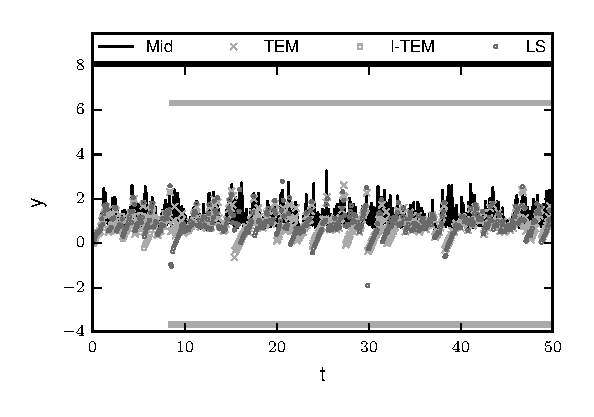
\includegraphics{Tretyakov}
		\caption{
			Numerical solution of SDE \eqref{eqn:SDETretyakov} using the I-TEM 
			\eqref{eqn:Increment-Tamed}, \SM method \eqref{eqn:TreyakovLSMethod}  and TEM-S \eqref{eqn:TEM-Sabanis}
			with $h=\num{0.1}$, the reference solutions is a Midpoint rule approximation with $h=\num{e-4}$
			}
		\label{fig:Tretyakov}
	\end{figure}
\subsection{Vector SDE}
{\textbf{Example 1.}}
Now we compare the order of convergence
and the run time of the \SM method withthe TEM scheme as in \cite{Hutzenthaler2012a}. That is,
we consider a  Langevin equation under  the $d$-dimensional potential 
$U(x)= \frac{1}{4}|x|^4 - \frac{1}{2}|x|^2$, and $d$-dimensional Brownian additive noise. The corresponding
SDE reads
\begin{equation}\label{eqn:SDELangevinHutz}
dy(t) = 
\left(
y(t) - |y(t)| \cdot y(t)
\right)dt
+dW(t), \qquad y(0)=0.
\end{equation}
This model describes the motion of a Brownian particle of unit mass immersed on the potential $U(x)$. 
Taking $a_j(x):=1-|x|$ and $b_j=0$, $j\in 1\dots d$ on we obtain the \SM method
\begin{equation}\label{eqn:LangevinLSMethod}
	Y_{k+1} = \diag
	\left[		
		\exp(h a_1(Y_k)), \dots, \exp(ha_d(Y_k)) 
	\right] 
	Y_k+
		\Delta W_k
\end{equation}
\Cref{tbl:OrdersLS} shows the root means square errors which is calculated as follows
\begin{equation}
	\sqrt{\EX{|Y_N - y(T)|^2}} = 
	\frac{1}{M}
	\left(
	\sum_{i=1}^M
		|y_i(T) - Y_{N,i}|^2	
	\right)^{1/2},
\end{equation}
at a final time $T=1$ over a sample of 
$M$ =\num{10000} trajectories of the TEM, \SM  and BEM solutions of SDE \eqref{eqn:SDELangevinHutz} 
with dimension $d=10$.  We consider the TEM solution with step $h=2^{-19}$ as reference solution. 
The TEM is faster and almost equal accurate than the LS method.

In some application as in Browninan Dynamics Simulations \cite{Cruz2012}, the dimension of a SDE
increases considerable the complexity and computational cost --- this prohibits the use of implicit methods.
\Cref{fig:TimeVsDimension} shows this (for SDE\eqref{eqn:SDELangevinHutz}): the runtime of BEM depends on 
dimension in a quadratic way , while the \SM and TEM depends on linear form.     
\begin{table}[t]
	\centering
	\begin{tabular}{lllllll}
		&        TEM &        	& LS		&           & BEM		 &         \\
		\toprule
		h		& ms-error	 & ECO 		& ms-error	& ECO		& ms-error	 &	ECO	  \\
		\midrule
		$2^{-2}$	& \num{1.70388}    & ---------		& \num{1.55394}		& ---------		& \num{1.38157}	& 
		--------- \\
		$2^{-3}$	& \num{1.16977}    & \num{0.5426}   & \num{1.10775}    & \num{0.488299} & \num{1.05309}	& 
		\num{0.391671} \\ 
		%$2^{-4}$	& \num{0.80253}    & \num{0.543601} & \num{0.783425}   & \num{0.499765} & \num{0.765585}& 
		%\num{0.46}     \\
		%$2^{-5}$	& \num{0.555121}   & \num{0.531752} & \num{0.54843}    & \num{0.514486} & \num{0.541855}& 
		%\num{0.498656} \\
		%$2^{-6}$   & \num{0.391732}   & \num{0.502937} & \num{0.389328}   & \num{0.494323} & \num{0.387508}& 
		%\num{0.483682} \\
		$2^{-7}$	&\num{0.27895}     & \num{0.489861} & \num{0.277957}   & \num{0.486126} & \num{0.276895}& 
		\num{0.484885} \\
		%$2^{-8}$	& \num{0.197226}   & \num{0.500153} & \num{0.196916}   & \num{0.497278} & \num{0.196837}& 
		%\num{0.492338} \\
		%$2^{-9}$	& \num{0.140522}   & \num{0.48906 } & \num{0.140456}   & \num{0.487466} & \num{0.140339}& 
		%\num{0.488091} \\
		%$2^{-10}$	& \num{0.0997332}  & \num{0.494646} & \num{0.0997064}  & \num{0.494358} & \num{0.0996544}& 
		%\num{0.493906  \\
		$2^{-11}$	& \num{0.0701043}  & \num{0.508572} & \num{0.0700918}  & \num{0.508439} & \num{0.070075} & 
		\num{0.508034} \\
		%$2^{-12}$	& \num{0.0496343}  & \num{0.498166} & \num{0.0496286}  & \num{0.498075} & \num{0.0496228}& 
		%\num{0.497898} \\
		%$2^{-13}$ 	& \num{0.0349302}  & \num{0.506861} & \num{0.0349278}  & \num{0.506797} & \num{0.0349242}& 
		%\num{0.506776} \\
		%$2^{-14}$	& \num{0.0248682}  & \num{0.490176} & \num{0.0248688}  & \num{0.490035} & \num{0.0248659}& 
		%\num{0.490057} \\
		$2^{-15}$	& \num{0.0173921}  & \num{0.515871} & \num{0.0173917}  & \num{0.515943} & \num{0.0173913}& 
		\num{0.515804} \\
		%$2^{-16}$	& \num{0.0122781}  & \num{0.502343} & \num{0.0122783}  & \num{0.502289} & \num{0.0122776}& 
		%\num{0.502336} \\
		%$2^{-17}$	& \num{0.00877132} & \num{0.485219} & \num{0.00877133} & \num{0.485239} & 
		%\num{0.00877136}&\num{0.485156} \\
		$2^{-18}$ 	& \num{0.00617193} & \num{0.507072} & \num{0.00617201} & \num{0.507055} & 
		\num{0.00617195}&\num{0.507074} \\
		\bottomrule
	\end{tabular}
	\caption{
		Mean square errors and the experimental convergence order (ECO) for the SDE \eqref{eqn:SDELangevinHutz} with 
		a TEM with $h = 2^{-19}$ as reference solution.
	}\label{tbl:OrdersLS}
\end{table}
\begin{figure}[t]
	\centering
	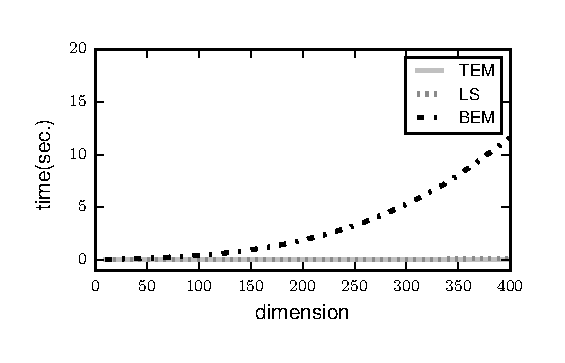
\includegraphics{TimeVsDimension}
	\caption{
		Runtime calculation of $Y_N$ with $h=2^{-17}$, using the BEM,  \SM and TEM methods for 
		SDE \eqref{eqn:SDELangevinHutz}.
	}
	\label{fig:TimeVsDimension}
\end{figure}

	
{\textbf{Example 2.}}
	\citeauthor{Hutzenthaler2012a} improve convergence of the Euler method by taming the drift increment term with 
	the factor
	$
	\frac{1}{1 + h |f(Y_k)|},
	$
	as consequence, the norm of  
	$
	\frac{h f(Y_k)}{1 + h |f(Y_k)|},
	$ is bounded by 1, which  controls the drift contribution of the TEM method at each step. This idea works very well
	over SDEs with drift contribution and initial condition that are comparable with this bound. However, we observed
	that on models where the	drift contribution has other scales, the TEM over damps the drift contribution. To fix
	ideas, we consider the	stochastic model reported in \cite{Dalal2008},
	\begin{align}\label{eqn:StochasticHIVDynamics}
	dy_1(t) &=
	\left(
	\lambda -\delta y_1(t) - (1 - \gamma) \beta y_1(t) y_3(t)
	\right)dt
	-\sigma_1 y_1(t) dW^{(1)}_t, 
	\notag \\
	dy_2(t) &= 
	\left(
	(1- \gamma) \beta y_1(t) y_3(t) - \alpha y_2(t) 
	\right)dt
	-\sigma_1 y_2(t) dW^{(1)}_t, 
	\\
	dy_3(t) & = 
	\left(
	(1 - \eta) N_0 \alpha y_2(t) 
	-\mu y_3(t)
	-(1 - \gamma ) \beta y_1(t) y_3(t) 
	\right)dt
	- \sigma_2 y_3(t) dW^{(2)}_t.
	\notag
	\end{align}	
	\begin{figure}[h!]
		\centering
		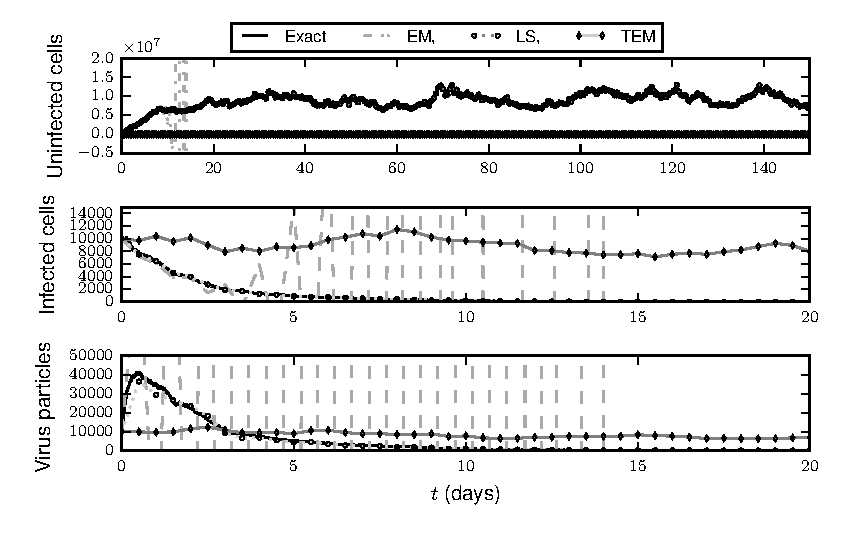
\includegraphics{InternalHIVDynamics5e-1}
		\caption{
			Likening between BEM, \SM, TEM approximations for SDE \eqref{eqn:StochasticHIVDynamics} with
			$\gamma = \num{0.5}$,
			$\eta = \num{0.5}$,
			$\lambda = \SI{1e6}{\per\cubic\deci\meter\per\day}$,
			$\delta = \SI{0.1}{\per\day}$,
			$\beta = \SI{1e-8}{\cubic\deci\meter\per\day}$,
			$\alpha = \SI{0.5}{\per \day}$,
			$N_0= \SI{100}{per cell}$,
			$\mu = \SI{5}{\per\day} $,
			$\sigma_1 = \num{0.1}$,
			$\sigma_2 = \num{0.1} $,
			$y_0 = (\SI{10000}{\per\cubic\deci\meter}, \SI{10000}{\per\cubic\deci\meter}, 
			\SI{10000}{\per\cubic\deci\meter})^T$,
			$h=\num{0.5}$.
			Here the reference solution means a BEM simulation
			with the same parameters but with a step-size $h=\num{1e-5}$.
		}
		\label{fig:InternalHIVDynamics5e-1}
	\end{figure} 
	Using a Linear Steklov formulation, we rewrite the drift coefficient as in
	\eqref{eqn:AlternativeConstruction} where 
	\begin{align}
		a_{1}(Y_k)) &:= 
			-\left(
				\delta + (1 - \gamma) \beta Y_k^{(3)}
			\right),		
			& b_1(Y_k^{(-1)}) &:= \lambda, 
			& E_1&:= \{ (x,y,z)\in \R^3: z=0\},
		\notag
		\\
		a_{2}(Y_k) &:= -\alpha,
			&b_2(Y_k^{(-2)}) & :=
			(1-\gamma) \beta Y_{k}^{(1)} Y_{k}^{(3)}, 
			&E_2&:=\emptyset,
		\notag
		\\
		a_{3}(Y_k) &= 
		-
		\left(
			\mu + (1- \gamma) \beta Y_{k}^{(1)}
		\right),
		\qquad
	%
		&b_{3}(Y_k^{(-3)}) &:= 
		\left(
			1 - \eta 
		\right)
		N_0 \alpha Y_{k}^{(2)}, 
		& E_3&:= \{ (x,y,z)\in \R^3: x=0\}.
		\notag			
	\end{align}
	 Then  the LS method \eqref{m1} for the stochastic model \eqref{eqn:StochasticHIVDynamics} is defined by
		\begin{align}
		A^{(1)}&:=
		\begin{pmatrix}
		e^{ha_1(Y_k)}	&	0	&0 \\
		0	&e^{ha_2(Y_k)}	&0\\
		0	&0				&e^{ha_3(Y_k)}
	\end{pmatrix},
%	
	\notag
	\\
	%	
	A^{(2)}&:=
	\begin{pmatrix}
			h\Phi_1(Y_k)\1{E_1^c}	&0	&0\\
			0 & 
			\left(\displaystyle
					\frac{e^{-h\alpha} - 1}{\alpha}
			\right)\1{E_2^c} & 0\\
			0	&0
			& h\Phi_3(Y_k)\1{E_3^c}% + h \1{E_i} 
	\end{pmatrix}
	+h
	\begin{pmatrix}
		\1{E_1} & 0& 0\\
		 0 &\1{E_2}& 0\\
		0 & 0&	\1{E_3}
		\end{pmatrix}.
		\notag
\end{align}
	
\citeauthor{Dalal2008} in \cite{Dalal2008} simulates SDE \eqref{eqn:StochasticHIVDynamics} with parameters reported 
	in published literature.
	\Cref{fig:InternalHIVDynamics5e-1} shows a simulation path with same parameters. We observe how the TEM  
	oscillates around of initial condition while the \SM follows the reference solution.  


\section{Conclusions}
In this work we have extended the explicit Steklov scheme for  vector SDE by 
developing a new version  based on a 
linearized Steklov average. 
The Linear Steklov approximation is constructed on the basis that the drift function 
can be rewritten  in a linearized form and by formulation this approximation is unique. 
Moreover, strong order one-half convergence has been proved for our explicit 
linear method and we have presented  many applications for which the LS scheme can be formulated. 
Finally high-performance of the Linear Steklov method  have been analyzed for ...



% %
% %********************************************************************************************
% %				 Bibliography
% %********************************************************************************************
% 
% 	\pagebreak
% 	\section*{\refname}
\begin{thebibliography}{26}
\providecommand{\natexlab}[1]{#1}
\providecommand{\url}[1]{\texttt{#1}}
\expandafter\ifx\csname urlstyle\endcsname\relax
  \providecommand{\doi}[1]{doi: #1}\else
  \providecommand{\doi}{doi: \begingroup \urlstyle{rm}\Url}\fi

  
\bibitem[Appleby and Kelly(2010)]{Appleby2010}
J.~Appleby, C.~Kelly,
\newblock On the local dynamics of polynomial difference equations with fading
  stochastic perturbations,
\newblock Dynam. Contin. Discrete Impuls. Systems 17 (2010)
  401--430.


\bibitem[Beyn et~al.(2010)Beyn, Isaak, and Kruse]{Beyn2010}
W. Beyn, E. Isaak, R. Kruse,
\newblock Stochastic c-stability and b-consistency of explicit and implicit
  euler-type schemes,
\newblock preprint arXiv:1411.6961 (2014) 1--29.

\bibitem[Chan and Williams(1989)]{Chan1989}
T. Chan, D. Williams,
\newblock An `excursion' approach to an annealing problem,
\newblock Math. Proc. Cambridge Philos. Soc. 105 (1989) 169--176.


  \bibitem[Cruz et~al.(2012)Cruz, Chinesta, and R\'{e}gnier]{Cruz2012}
C.~Cruz, F.~Chinesta, G.~R\'{e}gnier.
\newblock Review on the brownian dynamics simulation of bead-rod-spring models
  encountered in computational rheology,
\newblock Arch. Comput. Methods Eng. 19 (2012) 227--259.

\bibitem[Dalal et~al.(2008)Dalal, Greenhalgh, and Mao]{Dalal2008}
N. Dalal, D. Greenhalgh,  X. Mao,
\newblock A stochastic model for internal hiv dynamics
\newblock J. Math. Anal. Appl.
  341 (2008) 1084--1101.

\bibitem[D\'{\i}az-Infante and Jerez(2015)]{Diaz-Infante2015}
S. D\'{\i}az-Infante, S. Jerez,
\newblock Convergence and asymptotic stability of the explicit Steklov method
  for stochastic differential equations,
\newblock J. Comput. Appl. Math. 291 (2016) 36--47.

\bibitem[Fine and Kass(1966)]{FineAIandKass1966}
A. I. Fine,  S. Kass,
\newblock Indeterminate forms for multi-place functions,
\newblock Ann. Polon. Math. 18 (1965) 59--64.

\bibitem[Giles(2008)]{Giles2008}
M. B. Giles,
\newblock Multilevel monte carlo path simulation,
\newblock Operations Research 56 (2008) 607--617.

\bibitem[Glasserman(2004)]{Glasserman2004}
P.~Glasserman,
\newblock Monte Carlo Methods in Financial Engineering,
\newblock Applications of mathematics: stochastic modelling and applied
  probability, Springer, 2004.
  
\bibitem[Guo et~al.(2014)Guo, Li, and Zhu]{Guo2014}
Q. Guo, H. Li, Y. Zhu.
\newblock The improved split-step $\theta$ methods for stochastic differential
  equation,
\newblock Math. Methods Appl. Sci. 37 (2014) 2245--2256.


% \bibitem[Halidias(2012)]{Halidias2012}
% Nikolaos Halidias.
% \newblock Semi-discrete approximations for stochastic differential equations
%   and applications.
% \newblock \emph{International Journal of Computer Mathematics}, 89\penalty0
%   (6):\penalty0 780--794, April 2012.
% 
% \bibitem[Halidias(2014)]{Halidias2014}
% Nikolaos Halidias.
% \newblock A novel approach to construct numerical methods for stochastic
%   differential equations.
% \newblock \emph{Numerical Algorithms}, 66\penalty0 (1):\penalty0 79--87, 2014.

\bibitem[Higham et~al.(2002)Higham, Mao, and Stuart]{Higham2002b}
D. J. Higham, X. Mao,  A. M. Stuart,
\newblock Strong convergence of euler-type methods for nonlinear stochastic
  differential equations,
\newblock  SIAM J. Numer. Anal. 40  (2002)  1041--1063.

\bibitem[Hutzenthaler et~al.(2010)Hutzenthaler, Jentzen, and
  Kloeden]{Hutzenthaler2010}
M. Hutzenthaler, A. Jentzen, and P. E. Kloeden,
\newblock Strong and weak divergence in finite time of euler's method for
  stochastic differential equations with non-globally lipschitz continuous
  coefficients,
\newblock Proc. R. Soc. Lond. Ser. A Math. Phys. Eng. Sci. 467 (2010) 1563--1576.


\bibitem[Hutzenthaler and Jentzen(2015)]{Hutzenthaler2015}
M. Hutzenthaler, A. Jentzen, 
\newblock Numerical approximations of stochastic differential equations with
  non-globally lipschitz continuous coefficients,
\newblock Mem. Amer. Math. Soc. 236 (2015).


\bibitem[Hutzenthaler et~al.(2011)Hutzenthaler, Jentzen, and
  Kloeden]{Hutzenthaler2009}
M. Hutzenthaler, A. Jentzen,  P. E. Kloeden,
\newblock Strong and weak divergence in finite time of euler's method for
  stochastic differential equations with non-globally lipschitz continuous
  coefficients,
\newblock Proc. R. Soc. Lond. Ser. A Math. Phys. Eng. Sci. 467 (2011) 1563--1576.


\bibitem[Hutzenthaler et~al.(2012{\natexlab{a}})Hutzenthaler, Jentzen, and
  Kloeden]{Hutzenthaler2012a}
M. Hutzenthaler, A. Jentzen,  P. E. Kloeden,
\newblock Strong convergence of an explicit numerical method for sdes with
  nonglobally lipschitz continuous coefficients.
\newblock Ann. Appl. Probab. 22 (2013) 611--1641.


\bibitem[Hutzenthaler et~al.(2013)Hutzenthaler, Jentzen, and
  Kloeden]{Hutzenthaler2012b}
M. Hutzenthaler, A. Jentzen,  P. E. Kloeden,
\newblock Divergence of the multilevel monte carlo euler method for nonlinear
  stochastic differential equations.
\newblock Ann. Appl. Probab. 23 (2013)  1913--1966.


\bibitem[Lamba et~al.(2007)Lamba, Mattingly, and Stuart]{Lamba2007}
H.~Lamba, J.~C. Mattingly, and a.~M. Stuart.
\newblock An adaptive euler-maruyama scheme for sdes: Convergence and
  stability,
\newblock IMA J. Numer. Anal. 27 (2007) 479--506.

\bibitem[Lawlor(2012)]{Lawlor2012}
Gary~R Lawlor,
\newblock A l'hospital's rule for multivariable functions.
\newblock \emph{arXiv preprint arXiv:1209.0363}, 2012.

\bibitem[Liu and Mao(2013)]{Liu2013a}
W. Liu and X. Mao,
\newblock Strong convergence of the stopped euler-maruyama method for nonlinear
  stochastic differential equations,
\newblock Appl. Math. Comput. 223 (2013) 389--400,  2013.


\bibitem[Mao(2007)]{Mao2007}
X. Mao,
\newblock Stochastic Differential Equations and Application,
\newblock Horwood Pub., 2007.


\bibitem[Mao and Szpruch(2013)]{Mao2013}
X. Mao, L. Szpruch,
\newblock Strong convergence and stability of implicit numerical methods for
  stochastic differential equations with non-globally lipschitz continuous
  coefficients,
\newblock J. Comput. Appl. Math.
  238 (2013) 14--28.
  
  \bibitem[Mao(2015)]{Mao2015}
X. Mao,
\newblock The truncated euler-maruyama method for stochastic differential
  equations,
\newblock J. Comput. Appl. Math. 290 (2015) 370--384.


\bibitem[Sabanis(2013)]{Sabanis2013}
S. Sabanis,
\newblock A note on tamed euler approximations,
\newblock Electron. Commun. Probab. 18 (2013) 1--10.

\bibitem[Sabanis(2015)]{Sabanis2015}
Sotirios Sabanis.
\newblock Euler approximations with varying coefficients : the case of
  superlinearly growing diffusion coefficients.
\newblock to appear in Ann. Appl. Probab. (2015)

\bibitem[Tretyakov and Zhang(2013{\natexlab{a}})]{Tretyakov2013}
M. V. Tretyakov, Z. Zhang.
\newblock A fundamental mean-square convergence theorem for sdes with locally
  lipschitz coefficients and its applications,
\newblock SIAM J. Numer. Anal. 51 (2013) 3135--3162.



\bibitem[Wang and Gan(2013)]{Wang2011}
X. Wang,  S. Gan.
\newblock The tamed milstein method for commutative stochastic differential
  equations with non-globally lipschitz continuous coefficients,
\newblock J. Difference Equ. Appl. 19 (2013) 466--490.


\bibitem[Zong et~al.(2014)Zong, Wu, and Huang]{Zong2014}
X. Zong, F. Wu, Ch. Huang,
\newblock Convergence and stability of the semi-tamed euler scheme for
  stochastic differential equations with non-lipschitz continuous coefficients.
\newblock Appl. Math. Comput. 228
  (2014)  240--250.


\end{thebibliography}
\end{document}
